\documentclass[a4paper, oneside]{discothesis}

% use utf8 instead of latin1 when using LaTeX in windows
\usepackage[latin1]{inputenc}
\usepackage[font={small}]{caption}
\usepackage{subfig}
\usepackage{listings}


%%%%%%%%%%%%%%%%%%%%%%%%%%%%%%%%%%%%%%%%%%%%%%%%%%%%%%%%%%%%%%%%%%%%%%%%%%%%%%%%%%%%%%%%%%%%%%%%%
% DOCUMENT METADATA

\thesistype{Master Thesis}
\title{Towards Datamarkets with Bitcoin}

\author{Francisc Nicolae Bungiu}
\email{fbungiu@student@ethz.ch}
\institute{Distributed Computing Group \\[2pt]
Computer Engineering and Networks Laboratory \\[2pt]
ETH Z�rich}

% You can put in your own logo here "\includegraphics{...}" or just comment the command
% \logo{}

\supervisors{Christian Decker, Dominic W{\"o}rner, Laura Peer\\[2pt] Prof.\ Dr.\ Roger Wattenhofer}

% You can comment the following two commands if you don't need them
% \keywords{Keywords go here.}
% \categories{ACM categories go here.}

\date{\today}

%%%%%%%%%%%%%%%%%%%%%%%%%%%%%%%%%%%%%%%%%%%%%%%%%%%%%%%%%%%%%%%%%%%%%%%%%%%%%%%%%%%%%%%%%%%%%%%%%

\begin{document}

\frontmatter % do not remove this line
\maketitle

\cleardoublepage

\begin{acknowledgements}
	I thank Lorem ipsum dolor sit amet, consetetur sadipscing elitr, sed diam nonumy eirmod tempor invidunt ut labore et dolore magna aliquyam erat, sed diam voluptua. At vero eos et accusam et justo duo dolores et ea rebum. Stet clita kasd gubergren, no sea takimata sanctus est Lorem ipsum dolor sit amet. Lorem ipsum dolor sit amet, consetetur sadipscing elitr, sed diam nonumy eirmod tempor invidunt ut labore et dolore magna aliquyam erat, sed diam voluptua. At vero eos et accusam et justo duo dolores et ea rebum. Stet clita kasd gubergren, no sea takimata sanctus est Lorem ipsum dolor sit amet.
\end{acknowledgements}


\begin{abstract}

\hspace*{12pt} In recent years, there has been a widespread expansion of data collection and complex methods to analyze such 
collected data. Everyone is constantly generating data by using a large range of computers, smartphones, and gadgets.
In addition, there is an emerging trend towards the Internet of Things technologies that consist
of billions of sensor nodes bridging the gap between the physical and the digital world, and creating massive amounts
of data, but with no incentive to share. 

	In order to provide an incentive for the sensor node owners to share the generated data, these sensor networks
have to initiate data markets that interested customers can subscribe to and pay for the acquired data. Bitcoin provides
an Internet-native payment mechanism and protocols on top of Bitcoin are able to support small payments and avoid 
high cumulated transaction processing costs.

	This thesis proposes a centralized secure scheme that allows data purchasing from any Internet-connected sensor
node using the Bitcoin payments. Based on micropayment channels to aggregate payments and minimize transaction fees, 
and on contracts between the protocol participants to minimize trust, the scheme allows human judgements to be taken
out of the loop and supports complete automation. 
\end{abstract}

\tableofcontents

\listoffigures

\mainmatter % do not remove this line

% Start writing here
\chapter{Introduction}

\hspace*{12pt} The Internet of Things (IoT) is a novel concept that has rapidly expanded in the latest years, refering to the
network formed by any physical object, embedded with sensors and connectivity - such as Radio-Frequency 
Identification (RFID) tags, sensors, smartphones, etc. - that enables such nodes to exchange
data. This technology allows these objects to be sensed and controlled remotely (IoT Survey), having a great
impact on the every-day life of users, and resulting in efficiency and financial benefits.

Sensor nodes with Internet connectivity enable attractive sensing applications in various domains, ranging from
health-care, security and surveillance, environmental monitoring, agriculture automation, energy consumption, transportation, etc.
(Sensing as a Service paper) introduces the concept of Sensing as a Service, in which a number of sensors offer
their generated data as a service to interested entities through a central operator in exchange for a pre-established
price quote. 

Most existing payment protocols for the Sensing as a Service model involve a third-party, which results in higher costs and reduced
efficiency. Another approach is to rely on Bitcoin, a decentralized electronic payment system. 
Bitcoin has at its root the blockchain, a transaction database that is shared by all network 
nodes. However, these solutions fail to address the scalability problem of Bitcoin: 
they rely on atomic operations that are completed directly on the blockchain, thus increasing its size and moving Bitcoin
towards centralization, since only a few nodes will be able to process a block. 

IoT has a huge economic potential and areas of application include: road surveillance - interested in road condition data generated by cars (Nericell, VTrack), 
weather forecast - in data sensed by private weather stations, transportation - paying per distance or number of bus stops, 
paying for Internet by used traffic, etc. 
In this manner, IoT entities can act as active participants in a self-created data market. However, it is still lacking
an efficient payment method and is limited by high transaction costs.

In this context, the project proposes a centralized, low-trust and secure scheme that allows and incentivizes sensor nodes
to share sensed data and get paid in exchange in bitcoins. The presented solution utilizes micropayment channels
to solve Bitcoin's scalability problem by bundling several small payments for each set of acquired data and only
publishing the final, aggregated transaction to the network. In order to confer a low-trust relation between the system 
entities, the protocol relies on contracts that pass the payment obligation down from the buyer to the central coordinator,
and then to the sensor node. In addition to the theoretical model, a proof-of-concept is built based on the Android built-in
sensors.

\section{Background}

In the following sub-sections, the background on the used concepts and sub-protocols is presented.

\subsection{Bitcoin}

\hspace*{12pt} Since its invention in 2008 [Satoshi paper], Bitcoin has grown into a global electronic payment system.
It uses peer-to-peer technology to transfer funds, with no need for a central authority such as a financial institution
and low transaction fees, making it an attractive alternative to traditional payment methods.
A proof-of-work system and cryptographic protocols are the building blocks of the protocol, with peers participating
in the network being responsible for processing transactions and issuing of bitcoins. 

\vspace*{5pt}
\begin{figure}[!ht]
  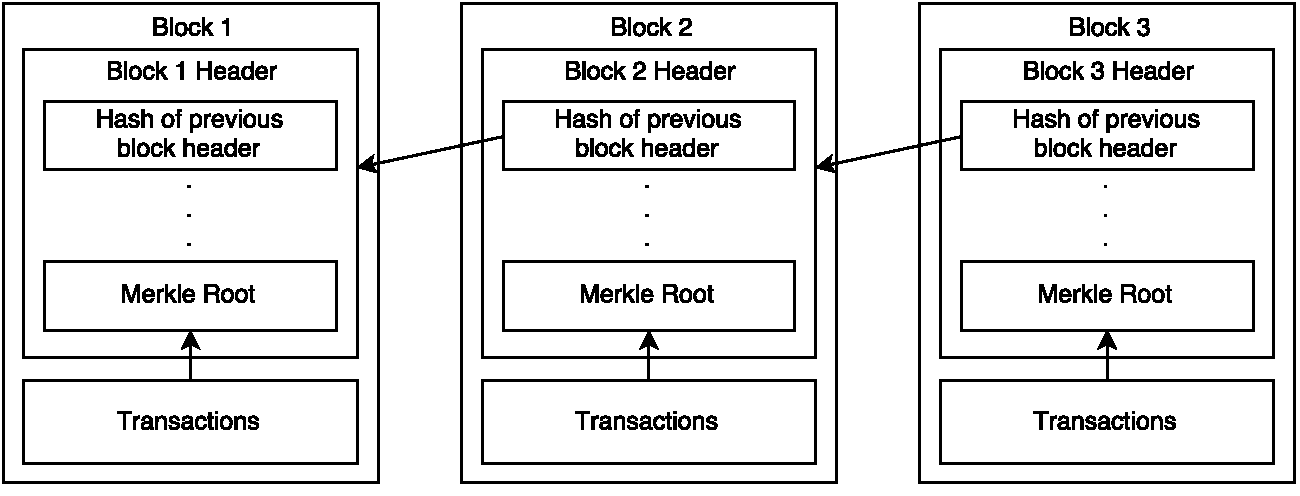
\includegraphics[width=\textwidth]{figures/Blockchain}
  \caption{A simplified representation of the Bitcoin blockchain.}
\end{figure}

Bitcoin relies on public key cryptography to authenticate transactions. Each peer in the network has one or more 
public and private key pairs that are stored in a file called a wallet. In order to support and authenticate transactions, 
an address is derived from the public key and is disclosed together with it to the participants.
In this cash system, transactions consist of one or more inputs (references to previous transaction outputs)
assigning the value of all inputs to one or more outputs. An output consists of a tuple of a specified
bitcoin amount, and an output script, called scriptPub. When trying to claim the funds, an entity must
create a signature script (scripSig), which has to satisfy the conditions in the previous output's pubkey scripts.
In most cases, the script only requires a signature matching the address, which proves the possession of the 
corresponding private key. The difference between the total input amount and the total
output amount in a transaction represents the transaction fee.
A peer holding a private key can sign a transaction spending some of its wallet's amount to some other address, and 
any other peer that sees this transaction can verify the signature using the peer's public key. In order to claim an
output, the payee must prove that it possesses the private key corresponding to the public key included as the destination
of the transaction. Thus, the available funds are represented by the amount of all unspent transaction outputs the peer possesses a private key for.

In order to be validated and accepted by the peers, 
a transaction needs to be broadcast to the network. Special network nodes, called miners, will then timestamp it by applying a hash function into
a continuously growing chain of hash-based proof-of-work. This forms a record, called the blockchain, containing
all transactions in Bitcoin ever made, that cannot be changed without redoing the entire proof-of-work.
The public ledger is distributed to all network peers and is crucial for protection against 
double spending and modification of older transactions. The proof-of-work performed in Bitcoin is based on HashCash POW [cite],
which means new blocks (containing one or more transactions) are only accepted into the ledger 
if the hash of the block header contains a specified number
of zeros as a prefix (adapted dynamically to produce bitcoins at a constant rate). 
The header of each block contains, among other data, a 4-byte nonce, that miners permute until 
the hash fulfills the criteria. Once it does, the new block is broadcast to the network and verified by the other peers
before being added to the blockchain. This PoW takes advantage of the random nature of cryptographic hashes, making it
impossible to modify the data to obtain predictable hashes. The computation, called mining, is incentivized through fees
that are earned by the nodes performing it.

\subsection {Micropayment channels}

\hspace*{12pt} Unlike traditional payment methods, Bitcoin transactions are very cheap in terms
of fees, but still have a considerable cost given the mining and storing they require. The context
of Internet of Things requires a high volume of small-value payments, thus the overall fees
might reach and surpass the value of the actual transactions. In addition to this, broadcasting
several transactions to the Bitcoin network in a very short time window will trigger network anti-flooding
algorithms, which will result in either the transactions being delayed or, even worse, not relayed. 
Last, the payee of such small transactions will end up with a wallet full of ``dust'', and spending
such money is expensive fee-wise.

To address these issues, the construct of payment channels was introduced in Bitcoin. After an initial
setup process between the two participants, the payer can start sending tiny payments to the other party
off the blockchain at high speed, without paying high transaction fees, in a trust-free manner.

\vspace*{5pt}
\begin{figure}[!ht]
  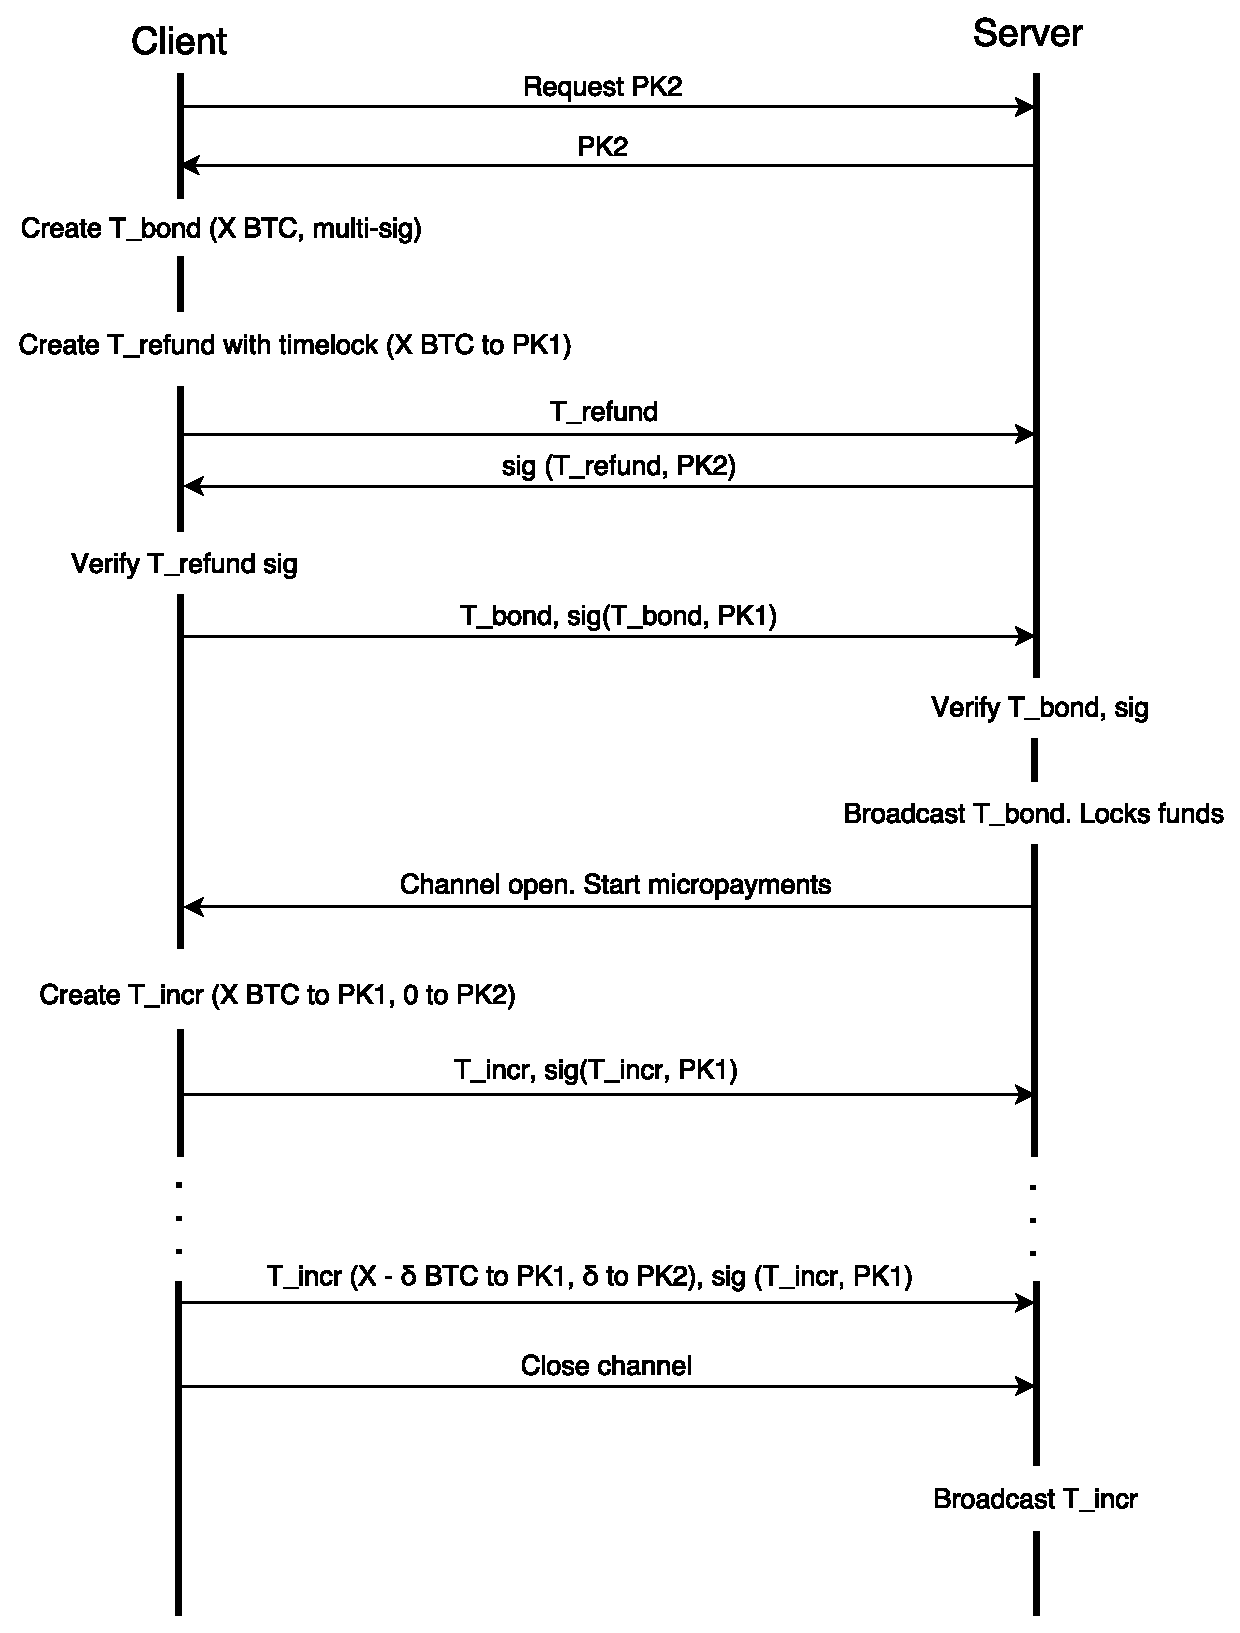
\includegraphics[width=\textwidth]{figures/MicropaymentSeq}
  \caption{Micropayment channel protocol: setting up the shared account (bond transaction), creating the refund 
  transaction, and updating the incremental payment transaction.}
\end{figure}

Consider a buyer that is interested in data generated by sensor nodes in a IoT network.
In exchange for the obtained data, it will pay the data provider in bitcoins. Since none of the
participants know each other, a zero-trust solution is necessary to reassure both the buyer that it will
not lose its bitcoins in case the sensor node does not provide the data, and that the sensor node will
not provide the promised service without getting remunerated. The construct works in two stages.
First, the buyer creates a multi-signature transaction, a shared account requiring signatures
of both participants to spend from it, that pre-allocates a certain amount of 
bitcoins for use in the channel. If the buyer signs and sends this bond transaction to the sensor node,
the node could simply broadcast it and keep the money hostage, thus the buyer keeps the transaction
private for now and creates another one, called a refund transaction, and sends it to the other
peer to sign it. This transaction refunds the
entire value to the buyer, but it time locked using the nLockTime feature of Bitcoin,
ensuring it will not become valid until some time in the future (channel lifetime). 
If the sensor node vanishes at any point, the buyer can then use the refund transaction 
to get all the money back at channel expiration time.

Once the refund has been signed by the sensor node, the buyer can safely send the signed bond transaction.
After verifying the signature, the server signs it as well and broadcasts it to the network, locking
in the money and opening the channel between the two parties. 

At this point, the work-and-pay cycles can begin. Initially, the buyer creates a new transaction
spending from the shared account and adds two outputs: one to its own address with the full amount, 
and one to the address of the payee. After signing it, the buyer sends it to the peer. 
When new data is requested from the data provider, the transaction is updated by the buyer, with increasing
value to the sensor node and decreasing value allocated to its own address. In each update cycle, the
transaction is signed and handed over to the other party. 
When the time comes and the buyer wishes
to close the channel, it notifies the sensor node, which in turn signs the transaction with the 
highest value alloted to it and broadcasts it to the network. This step closes the channel, unlocking
the buyer's remaining money and making the sensor's money available for spending. The buyer could be
tempted to broadcast an older transaction that gives less money to the sensor node than it deserved
for the provided data, but it is missing the sensor's signature. Thus, the construct of micropayment
channels prevents misbehavior from both parties.

\subsection{Hashed Time-Lock Contracts (HTLCs)}

\hspace*{12pt} Since the project proposes a three-component system in which payments need to be forwarded
from the buyer all the way to the data sensor nodes, a blockchain enforced contract needs to be set in place
in order to prevent the intermediaries from delaying or keeping these funds for themselves.

To create an HTLC, a special HTLC setup transaction is set up that can only be claimed 
by the final recipient {\it B}  of the payment using a previously created secret.
First, the payee {\it A} has to generate a secret {\it R} and hash it to obtain {\it H}. 
Then {\it H} and the recipient's Bitcoin address are directly transferred to the payer. 
At this step, all nodes on the  payment path between the sender and the recipient
need to create HTLC setup transactions connected to the output of a shared account 
using the provided hash H. The output of the HTLC setup contains a pubScript as shown in
\ref{fig:htlcpubscript}, which requires
a signature from both participants (first branch), or the next hop provides {R'} such that
it hashes to {\it H}.
Once all setup transactions are in place, the recipient {\it B}
can release {\it R} to claim the funds from the previous node. The secret is then revealed
step by step by all nodes on path all the way back to {\it A}, which completes the transfer.

\vspace*{5pt}
\begin{figure}[tbp]
  \centering
    \subfloat[HTLC pubScript.]{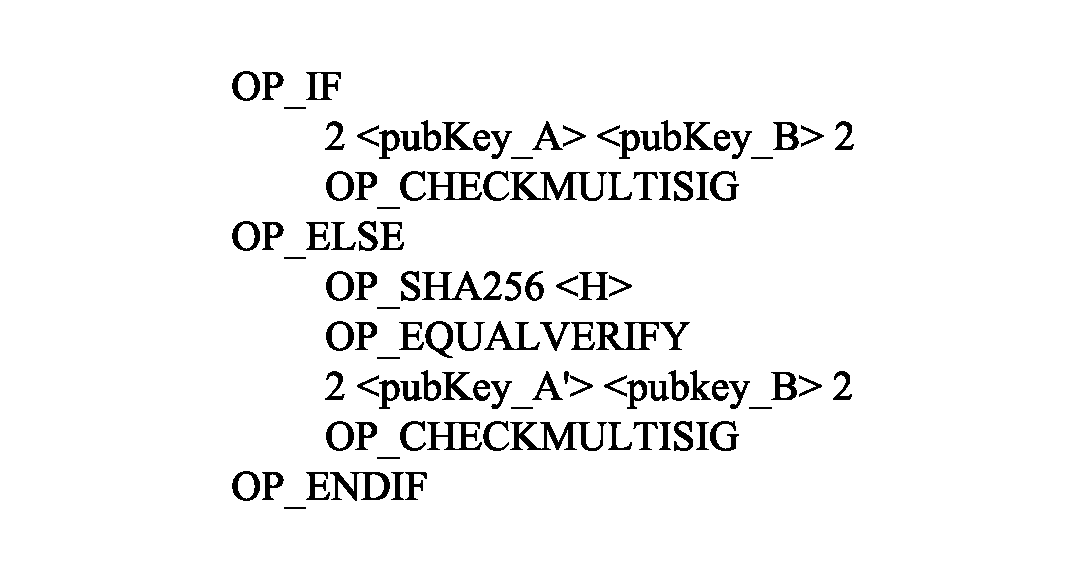
\includegraphics[width=0.5\textwidth]{figures/HTLCPubScript}
    \label{fig:htlcpubscript}}
    \subfloat[HTLC Transaction structure.]{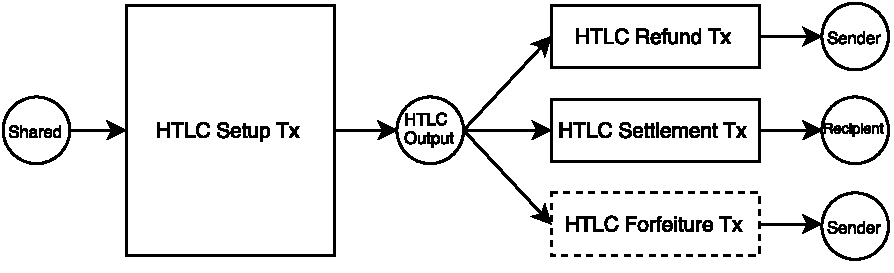
\includegraphics[width=0.5\textwidth]{figures/HTLCTxs}
    \label{fig:htlctxstructure}}
\end{figure}

To prevent the intermediaries from delaying the funds, stealing or keeping them hostage, 
HTLC refund, settlement and sometimes forfeiture transactions are created, all three types
claiming the HTLC output. 
The {\it HTLC refund} transaction is similar to the refund that is created in the micropayment
channel setup protocol, but has a higher time lock to give the sender enough time
to react, should the receiver not cooperate.
The {\it HTLC settlement} transaction guarantees the receiver it can pull the funds if it 
is in the posession of the secret. It is important for the sender to use different signing keys
{\it A} and {\it A'} for the two branches of the HTLC output. Otherwise, the receiver 
could simply reuse the signature of the settlement transaction in the if-branch and claim
the funds without ever revealing the secret, since the signature is valid for the entire pubScript.
Lastly, the {\it forfeiture transaction} addresses the case in which the sender and the
receiver agreed to void the HTLC and remove the output. If the receiver comes in possession
of the secret at a later stage, it still has the signed settlement transaction that it 
could simply broadcast and steal the bitcoins. Because of this, every time the receiver
backs off from the HTLC, it creates and hands over a forfeiture transaction that transfers the bitcoins
back to the sender. Should the receiver broadcast an older setup transaction,
the sender can simply use the forfeiture to get the money back.

%Notes: 
% reputation systems
% bitcoin soft-fork from Lightning to secure the protocol
% Android device can encrypt data with the buyer's pubkey  + secret : onion, or ECDSA

\section{Related work}

\hspace*{12pt} Following the expansion trend of the Internet of Things technologies, there has been an increasing interest in 
creating secure payment protocols that allow customers to acquire sensor data efficiently. 

(IoT based on the Protocol of Bitcoin paper) introduces a new low-trust E-business architecture that is tailored 
for IoT. This architecture is based on Bitcoin, eliminating the need for a 
third-party in the process. In order to make a payment and receive the data in exchange, the buyer and the data provider 
make an offer-proposal exchange, then build a transaction that spends the required amount and publish it to the network. 
A similar approach is proposed in (When Money learns to fly), where the encrypted data is directly included in the 
blockchain after a payment is made, which only the buyer in possession of the corresponding private key can decrypt.
In both approaches, all transactions, no matter how small, need to be published to the network, which results in high 
cumulated fees and time-wise inefficiency, thus being directly affected by the scalability problem of Bitcoin (cite).

Work has also been done on micropayment protocols that reduce fee costs.
Amazon Flexible Payment Service uses a central provider that aggregates 
clients' micropayments into macropayments that are flushed to the seller at specific times. This solution
does not provide anonymity, since the central provider can keep track of all payments, and moreover,
was discontinued on June 1, 2015.
Other protocols (Micropayments Revisited) involve a probabilistic approach. Using a selection rate {\it s}, it
discards all unselected micropayments and selects one with probability {\it s} that can be deposited for an amount
{\it 1/s} times bigger than the original amount. This should ensure everyone gets, on average, the expected amount. 
However, this solution lacks anonymity, requires PKI certificates and comes closer to a bet than an actual transaction.

The Architecture of Coupon-Based, Semi-off-Line Anonymous Micropayment System for Internet of Things - 
proposes an anonymous, semi-offline micropayment system for transactions in IoT. In this approach, an electronic
coin is obtained by iteratively applying a hash function to some initial seed, thus allowing the user to spend it
in fractions, by presenting a set of hash chain nodes to the vendor. 
The protocol is designed to meet the needs of IoT transactions, however, it has limited potential to be implemented because it does 
not rely on an existing financial institution. 
Another coupon-based system has been proposed by Rivest in [PayWord and MicroMint] and was improved by Payeras-Capella 
(An efficient anonymous...) to integrate anonymity and prevent users from exceeding their account limit. The drawback of the
latter is that the financial institution needs to be contacted directly before each payment, and any unspent value is lost
in favor of the financial institution. Wilusz (Requirements and general..) solves these issues by requiring a single 
contact with the financial institution at coin issue time and allowing the user to use unspent fractions in future transactions.
However, a clearing house is necessary to lock in the coin by the vendor, which increases transactions costs, 
and poses the risk of locking the coin indefinitely.

There have been some previous projects that utilize micropayment channels to pay in bitcoins in exchange for services. 
[Paying for Internet one byte] is a proof-of-concept allowing an access point to provide Internet access to 
untrusted users for bitcoins through a micropayment channel in a convenient manner. This way owners are incentivized
to open up their access points and users receive Internet services in return. Though the idea of using micropayment
channels for several small-valued transactions does address the scalability problem of Bitcoin, establishing micropayment
channels between all pairs of buyers and service providers is rather inefficient in the context of this project.

It is worth mentioning that there have been several proposals and ideas that can be exploited to support
trustless, instant, off-the-chain Bitcoin payments
on bitcointalk.org by Mike Hearn, Alex Akselrod, hashcoin, Meni Rosenfeld, cjp, Tier Nolan etc.

On the Contracts page of Bitcoin, Mike Hearn (https://en.bitcoin.it/wiki/Contract\#Example\_2:\_Escrow\_and\_dispute\_mediation) describes an idea
on how to trade with somebody with no trust involved, based on multi-signature transactions. The funds get locked in a shared account
controlled by at least two of the three participating parties: the client, merchant and mediator. If the transaction is successful
or a refund is agreed upon, the client and the merchant can move funds. If the trade fails, the client and the mediator can agree,
and a charge-back occurs. Finally, if the goods are delivered but the client does not want to fulfill its part of the agreement,
the mediator and the merchant agree and the merchant gets the client's money. Mike also proposed the idea of trading across
multiple currencies without a third party, and Tier Nolan formalized it in a protocol that allows the exchange atomically, using
time locks and hash commits.

cjp presented a draft that combines Bitcoin and Ripple to create a high-speed, scalable, anonymous, decentralized, low-trust
payment network. In this Bitcoin-specialized variation of the Ripple system, neighboring pairs
have a shared account that is partly allocated to one of them, and the rest to the other, as agreed
between the two, which lowers the needed trust. Using sequence numbers to update this transaction
as payments in the network are made and lock times to prevent blocking the money indefinitely. 

Meni Rosenfeld proposed
a simple way of reusing existing micropayment channels instead of establishing new ones if a path between
the payer and the payee already exists. The intermediaries would then only be trusted with the amount of a single payment
from a single buyer. 

Alex Akselrod - Extensible Scalable Coopetitive High Availability Trade Optimization Network - built a proof-of-concept
for chained micropayment channels with two-phase commits. The original micropayment channel payment scheme is modified
to allow sending funds through intermediaries. Suppose Alice, Carol, and Bob have previously set-up micropayment channels
pairwise, in the given order. If Alice wants to send bitcoins to Bob through Carol, Bob first creates
a random secret R, hashes it and sends the commit hash to Alice out-of-band. Then Alice can update the values on the
channel with Carol using the commit hash, and Carol can do the same on the channel with Bob. In order to claim the money,
Bob has to reveal the secret to Carol, and Carol can then reveal the secret to Alice up the path to receive her funds.
Thus, this proposal enables friend-to-friend, instant, off-blockchain, trustless payments of arbitrary size using Bitcoin
micropayment channels.

Peter Todd's proposal in Hub-and-Spoke Payments provides the an efficient way for establishing micropayment
channels between peers with a central hub. This central entity plays the role of a router, basically fowarding
payments from the payer to the payee. Suppose Alice and Bob have previously established micropayment channels with
the hub. If Alice wishes to send bitcoins to Bob, she should normally establish a new micropayment channel with him.
However, both of them have channels opened with the hub, so Alice can send the funds to the hub, and the hub can then
forward the payment to Bob. Using Hub-and-Spoke payments, payments between buyers and service providers with a central
coordinator can be made efficiently, saving costs in terms of fees. However, the forwarding process should be enforced and secured,
part that is noted in the proposal, but without specifying an actual way to do so. 

The Lightning Paper presents a promising solution to Bitcoin's scalability problem and provides a way to
securely forward payments on a path of peers through blockchain enforced contracts. 
It solves the issue by using timelocks on a network of micropayment channels combined with Hashed Timelock Contracts (HTLC) 
- recipient generates random data R, hashes it to produce H and sends H to the sender of funds, together with its bitcoin address. 
Sender routes its payment to the receiver and when an updated transaction is received, the recipient may elect to redeem the 
transaction by disclosing the random data R (which pulls the funds from the sender).
With the introduction of a new sighash
type which solves malleability, the proposed protocol allows offchain transactions between untrusted parties with fully enforceable
contracts, making Bitcoin scale to billions of users.

For the sake of completeness of this literature review, we mention the TilePay project, which promises a decentralized
payment system based Bitcoin for real-time access to IoT sensors, based on micropayments. In a partnership
with Cryptotronix, TilePay wants to enable cryptocurrency payments to IoT devices. However, since the announcement
in December 2014, no work or detailed information on how they would achieve that has been published.

\chapter{Design}

\section{Requirements}

\hspace*{12pt} For the presented use case, a scheme that enables sensor nodes in an Internet-of-Things network to shared sensed data and 
get paid in exchange must meet the following requirements:
\begin{itemize}
 \item Provide an entity that the node can register sensor type availability to.
 \item Provide an entity that buyers can query for available data and that can provide sensor node contact
 information
 \item Scalability: avoid broadcasting all micro-transactions to the blockchain
 \item Efficiency (and speed): fast communication between components, payments and data should be confirmed and received instantly
 \item Secure: end-to-end security of the payments
 \item Anonymous: linking of buyers and sellers and identification across sessions should not be possible.
\end{itemize}

\section{System Overview}

\hspace*{12pt} The design of the payment system achieving the requirements above comprises three major components:
one component consists of several sensor data providers (IoT sensor nodes, Android phones
running specialized app, etc.), one central hub that plays an essential role in sensor node discovery
and payment and data relaying, and a third component, consisting of data buyers. The communication
between the buyers and the hub, and between the hub and the sensor nodes is done through TCP links.

\begin{figure}[!ht]
  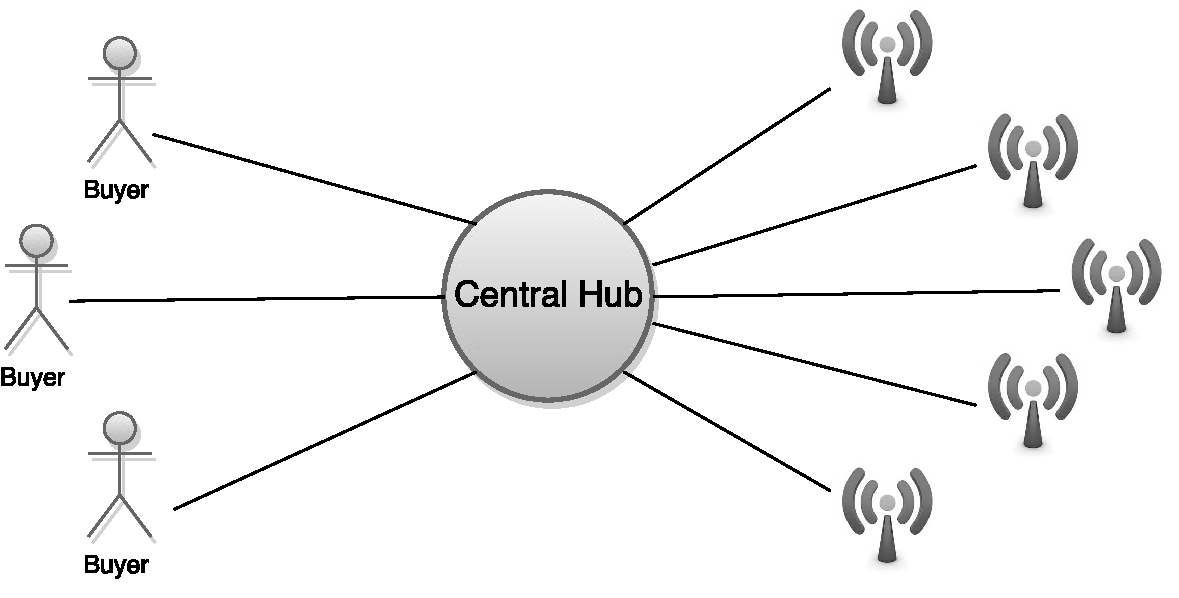
\includegraphics[width=\textwidth]{figures/SystemOverview}
  \caption{System overview: buyers, central hub, and sensor nodes.}
\end{figure}

\section{System components}

\hspace*{12pt} In this subsection, each of the three system components is presented in more detail.

\subsection{Sensor nodes}

\hspace*{12pt} In order to participate in the system, the sensor nodes need Internet connectivity to establish 
TCP connections to the central hub. The node then initiates the establishment of a long-term micropayment channel. 
Once the setup is complete, the availability of the sensors is signaled to the hub, which registers them
accordingly for future buyer queries.

\subsection{Buyers}

\hspace*{12pt} This component consists of a simple interface connecting to the hub through a TCP connection. First,
a micropayment channel is established with the central hub. After this initial step, the buyer
can run queries such as:
\begin{itemize}
 \item Node statistics: offer information on the number of connected sensor nodes. 
 \item Sensor statistics: offer information on the types of sensors that are available for purchasing.
 \item Select queries: allow buyers to query for a certain type of sensor data and inform them
 on nodes this data is available on, together with pricing information.
 \item Buy queries: allow buyers to purchase a set of data for a certain sensor type from a selected node.
 This query will return the asked data set.
\end{itemize}

\subsection{Central Hub}

\hspace*{12pt} At the heart of the system lays the central hub. According to the requirements, the hub acts as a coordinator
, payment forwarding medium and meeting point between the buyers and the data providers. It establishes micropayment
channels with all sensor nodes sharing their data and all buyers. On the other hand, each of the other two components
only need to keep one micropayment channel open, with the central hub.

When a new data provider connects to the central entity, it establishes a TCP connection and sets up a new 
micropayment channel between two. That is, the hub has to lock in a certain amount for a longer time interval 
({\it 30} days, for example). Assuming numerous data providers, the hub is required to have a high amount of bitcoins
to pre-allocate in each established channel to run the entire system.

To support the two types of connection, the hub is running two servers, 
providing specialized handlers that communicate with each sensor node and buyer connecting to it. 
A driver component coordinates the two subcomponents, book-keeping connected nodes and buyers, and forwards messages
between the buyers and nodes.

\section {Achieving the requirements}

\subsection{Achieving Scalability and Efficiency}

\hspace*{12pt} In order to achieve scalability and efficiency, there are two important factors that need to be taken
into account: the inherent scalability issue of Bitcoin and the number of peer pairs that need
to interact to successfully get payments from buyers to the sensors.

Since sensor nodes are exchanging small sets of sensed data in exchange for bitcoins, individual payments
made by the buyer tend to be of very small amounts. Therefore, creating new transactions for each
such payment would have a very high overhead in terms of fees, which reduces the incentive for
both the buyers and the sensor nodes to participate in the protocol. A high volume of transactions
would also delay the transactions being confirmed on the Bitcoin network. To address these
issues, the proposed system will rely on the previously introduced micropayment channels. 
This mechanism will allow, after a preliminary setup between the parts that wish to transact,
to instantly send small amounts of bitcoins off the blockchain, bundling and publishing them to the
network only at the end of a specified time window. Thus, both scalability of Bitcoin and efficiency
of payments are achieved.

One issue that comes with using micropayment channels in the proposed context 
is that its set-up phase takes a considerable time (approximately 10 minutes, until the bond transaction
is confirmed by the network). Thus, setting up a channel between all buyers and nodes becomes 
very inefficient time-wise and causes a lot of overhead on the network since all connections need
to be maintained for the lifetime of the channel.
On the other hand, if the buyers and the sensors
have previously established a channel with a central entity as in the hub-and-spoke model (cite), 
each will have a single set-up to wait for and a single channel 
connection to maintain. To better illustrate the performance improvement, suppose the system runs
{\it X = 100} buyers and {\it Y = 100} data providers. By using the initial idea, {\it X*Y = 10.000} 
channels  need to be established and maintained. With the hub-and-spoke model, however, 
{\it X + Y = 200} channels will suffice (factor of {\it 50}).

Last, adding a single central entity may affect the scalability of the system when the number of 
data providers and buyers increases, becoming a performance bottleneck. 
However, the concept of a central hub should be rather
treated as a central cloud, which can contain several machines maintaining the connections,
channels, available sensor data, and load balancers that distributed the work across the available
machines.

\subsection{Achieving Security}

\hspace*{12pt} To achieve efficient end-to-end security on the path between the buyers and the data providers, 
pre-established micropayment channels are combined with HTLCs. This ensures that
all nodes on the payment path receive their funds and if funds are delayed or taken hostage,
a maximum penalty will incur for the defecting node. The method is first presented for
neighboring nodes, then extended for full paths.

\subsubsection{Between neighboring nodes}

\vspace*{5pt}
\begin{figure}[!ht]
  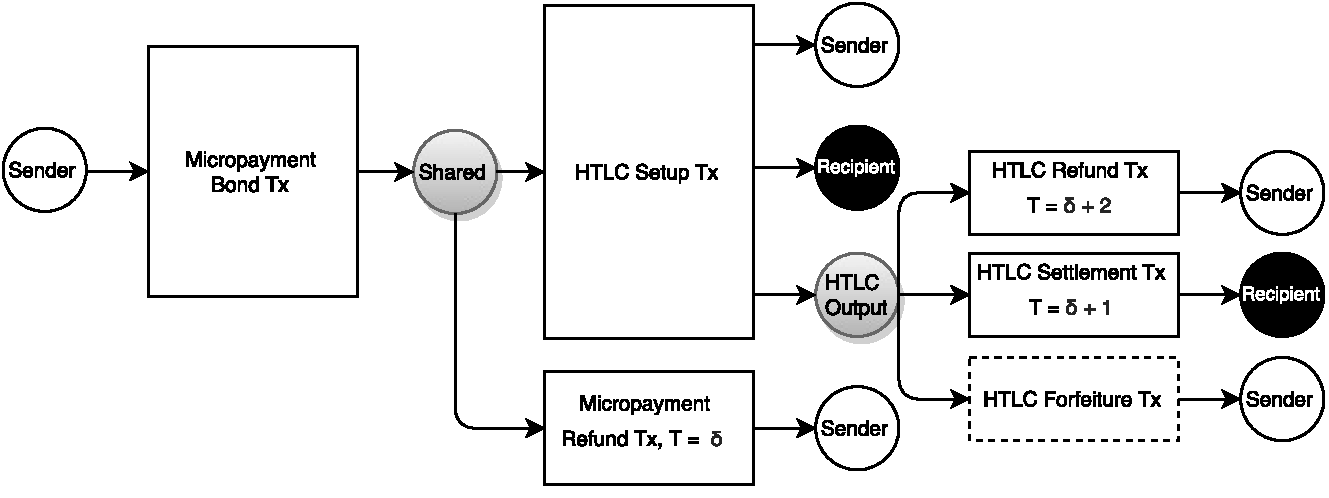
\includegraphics[width=\textwidth]{figures/MicroHTLC}
  \caption{Micropayment channels with HTLCs for end-to-end security on payment paths}
\end{figure}

\hspace*{12pt} First, the two neighboring nodes have to set up a shared account 
(multi-signature transaction) between the two of them. Once the bond
transaction is broadcast to the network, the funds are locked in and the micropayment channel is 
opened. Initially, an HTLC setup transaction spending the shared output is created, allocating 
the full channel amount to the sender, and $0$ to the recipient. When a new payment is created,
instead of directly increasing the amount which the recipient, an HTLC output with the
payment amount is added to the HTLC setup transaction, which requires a secret $R$, 
known only by the recipient, to be revealed in order to claim the payment. 
As previously explained, the HTLC output is spent by three
transactions: the HTLC refund, settlement and forfeiture transactions. 

In order to be able to claim the HTLC output, the receiving party has to broadcast the HTLC
setup transaction before the channel refund transactions becomes valid at $ T = \delta $.
If the sender still tries to broadcast the channel refund, the transaction would be rejected
since it double-spends the multi-signature output of the bond transaction. Once the HTLC setup
transaction is confirmed by the network, the HTLC output becomes available. 
If the recipient has the secret, it has time until $ T = \delta + 1$ to commit the settlement
transaction. On the other hand, if it does not, it can simply agree with the sender to remove the
HTLC output (voiding the payment), and hand it over a forfeiture transaction that guarantees it will
not use an older HTLC setup transaction version, should it receive the secret at a later time.
Thus, the HTLC settlement transaction needs a time lock $ T = \delta + 1$, higher than the latest time the setup transaction
can be committed, such that the forfeiture transaction can be safely broadcast within the time
window the HTLC output is committed and it being spent by the settlement transaction. Last,
if the settlement transaction is not used by time $T = \delta + 2$, the sender will get its funds
back using the HTLC refund transaction.

The main use of the presented protocol is to keep as many transactions as possible off the blockchain.
In order for this to work, the recipient, instead of broadcasting the settlement transaction to reveal the 
secret and claim the money, it can simply reveal it directly to the sender. This way, both parties
can agree on removing the HTLC output from the setup transaction, updating the output allocated to the
recipient with the amount of the HTLC. If the recipient chooses to void the HTLC instead, it can
sign a forfeiture transaction and hand it over to the sender, guaranteeing the sender that
it will not use an older setup transaction. By doing this, the HTLC output is again
removed, and its value is added back to the output of the sender.

\subsubsection{On full path}

\hspace*{12pt} To achieve end-to-end security on the full path between the buyers, central hub, 
and sensor nodes, the protocol above is extended. First, the buyer and the sensor node 
have to establish micropayment channels with the central hub. In order to make a payment, 
the buyer has to first make a request to the final recipient, the sensor node, through the hub, 
which generates a secret $R$, hashes it to obtain $H$, and sends $H$ back to the buyer. 
Using the received hash, the buyer opens a new HTLC flow with the central hub, by adding an 
HTLC output to the setup transaction spending from the shared account between the two. 
Once the process is complete, the hub then uses $H$ to open a corresponding HTLC flow with 
the sensor node. After this step, the sensor can release the secret to the hub to claim its money,
which can then use it to claim the funds from the buyer, closing the two HTLCs. This process
provides end-to-end security on the payment path.

\vspace*{5pt}
\begin{figure}[!ht]
  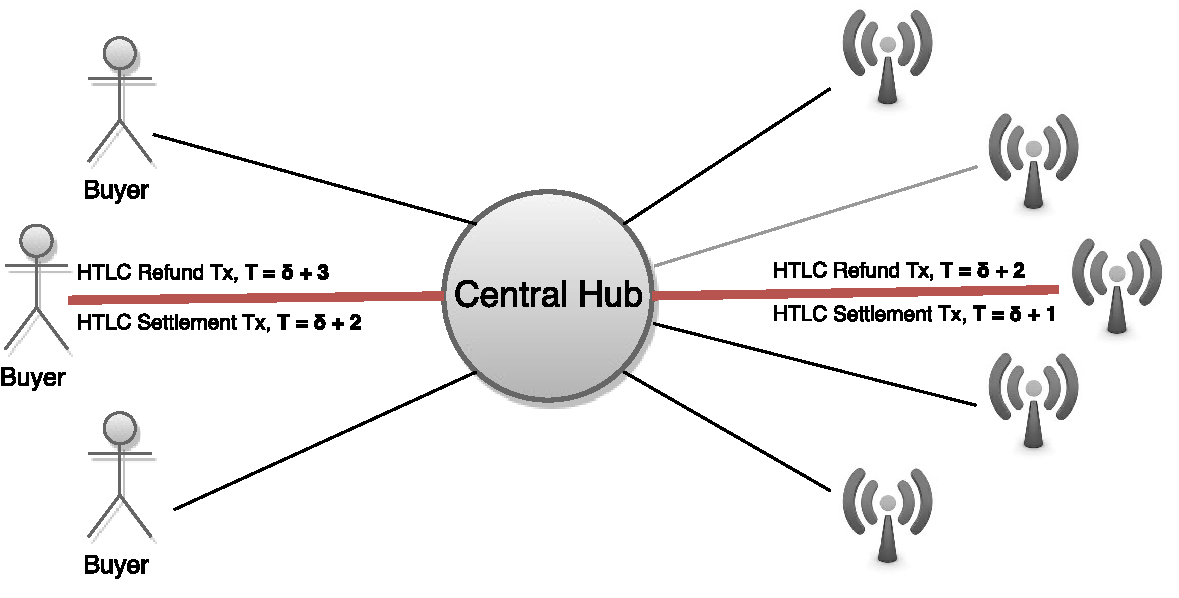
\includegraphics[width=\textwidth]{figures/FullMicroHTLC}
  \caption{Securing payment paths between buyer, hub, and sensor nodes with micropayment channels and 
  HTLCs}
  \label{fig:fullmicrohtlc}
\end{figure}

In order for the protocol to be fully secure in this two-hop payment scenario, the time locks of 
the HTLC refund and settlement transactions from the recipient up to the buyer need to be higher
than the ones from the previous hop (see \ref{fig:fullmicrohtlc}), such that no participant
can reveal the secret so late the upstream is not given the opportunity to claim its coins in time.

\subsection{Achieving Anonymity}

\hspace*{12pt} By design, the role of the central hub is to connect data buyers and sellers, and given that
the lifetime of the established micropayment channels are rather long, the hub can easily analyze
the data a buyer is interested in, build a profile and ultimately, identifying it. To address
the privacy issue, buyers could make use of a distributed 'onion' network, such as Tor,
open several, shorter-lived sessions, over several vantage points, 
and spread payments and data exchanges on these session when buying different sets of data. 
An additional precaution is to never reuse addresses across sessions. 
This way, profiling becomes more difficult,
and the hub can not link anymore buyers and data they have purchased through the system.

\chapter{Implementation}

\hspace*{12pt} The focus of this work is to propose a centralized, low-trust, and secure scheme that enables
IoT sensor nodes to share their data in exchange for bitcoins. The design chapter presented a solution 
that meets the system requirements. Following the introduced design, the Java implementation of a 
proof-of-concept based on the Android built-in sensor is presented in this chapter.

\section {API design}

\hspace*{12pt} The implementation of the system is based on {\it bitcoinj}, a Java library that allows users
to work with the Bitcoin protocol. Its features include maintaining a Bitcoin wallet, creating, sending and
receiving transactions, but also more advance constructs such as contracts and micropayment channels. 

From a high-level point of view, the system is designed according to the client-server architecture, 
in which each component is either a client or a server. The buyer component and the sensor subcomponent of the hub 
that are spending funds in exchange for a service are considered clients. On the other hand, the buyer subcomponent 
of the hub and the sensor node component providing data in exchange for bitcoins are considered servers. 

\vspace*{5pt}
\begin{figure}[!ht]
  \centering
  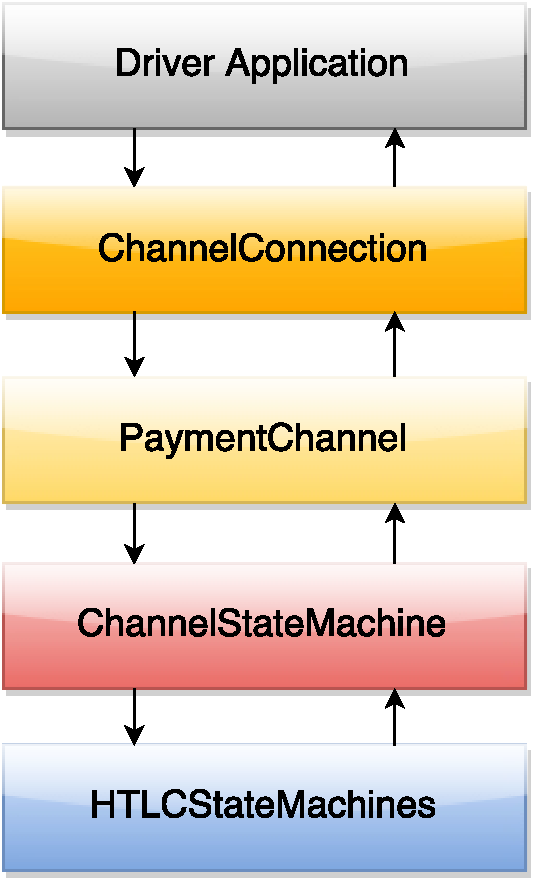
\includegraphics[width=7cm, height=10cm]{figures/LayeredAPI}
  \caption{Five-layered application architecture}
  \label{fig:layeredapi}
\end{figure}

From a logical point of view, each application relies on a layered design, which improves maintainability 
(easy to modify, test, debug, reuse layers), and performance. Layers exchange information through strict interaction.
This approach offers a rigorous separation of concerns and ensures that each layer only interacts 
with the one directly below. Each application is layered according to Figure \ref{fig:layeredapi}:
\begin{itemize}
  \item \textbf{Driver application layer.} This is the topmost layer representing an interface the users can directly
  make use of to access the functionality provided by the lower layers. Following the design patterns from 
  the {\it bitcoinj} library, the ListenableFuture class from the Google Guava library is used to register callbacks 
  in the Driver layer, so the application gets notified once a computation is complete.
  \item \textbf{Channel Connection layer.} This layer is responsible for reading and writing objects to the network.
  The functionality is provided by the {\it niowrapper} package of the {\it bitcoinj} library, which relies on 
  Java NIO: nonblocking, socket I/O. It also provides multiplexing, a technique used to monitor
  multiple I/O operations executing concurrently from a single thread, obtaining high performance and low latency.
  \item \textbf{PaymentChannel layer.} The middle layer is responsible for processing the messages that are received
  through the wire from the layer above, dispatching tasks to lower layer accordingly, receiving results from them,
  and finally constructing message replies and dispatching them to the connection layer. Micropayment channels are
  fully supported by the {\it bitcoinj} library; however, for this project, the package was rewritten to support
  HTLCs and simplified by removing the layer responsible for resuming channels in case of connection failure.
  \item \textbf{ChannelStateMachine layer.} This layer provides a state machine independent of any network protocol.
  It is the Bitcoin-aware layer: it constructs transactions, signs them, schedules refunds for future broadcasts
  to initiate, use, and safely close a micropayment channel.
  \item \textbf{HTLCStateMachines layer.} This layer provides one or more state machines that are responsible 
  for keeping track of the HTLC flow. By allowing several instances to run at the same time, concurrent payments
  are possible.
\end{itemize}

Both clients and servers adhere to the architecture above, with differences in functionality.
In the next subsection, the two component types are introduced in more detail. Their interaction
to run the proposed payment protocol is then described.

\subsection {Client}\label{client}

\hspace*{12pt} Figure \ref{fig:clientuml} the structure of the developed client component, containing its classes and their
relations, attributes, and operations. The classes and their responsibilities are described in a top-down
manner.

\begin{figure}
  \centerline{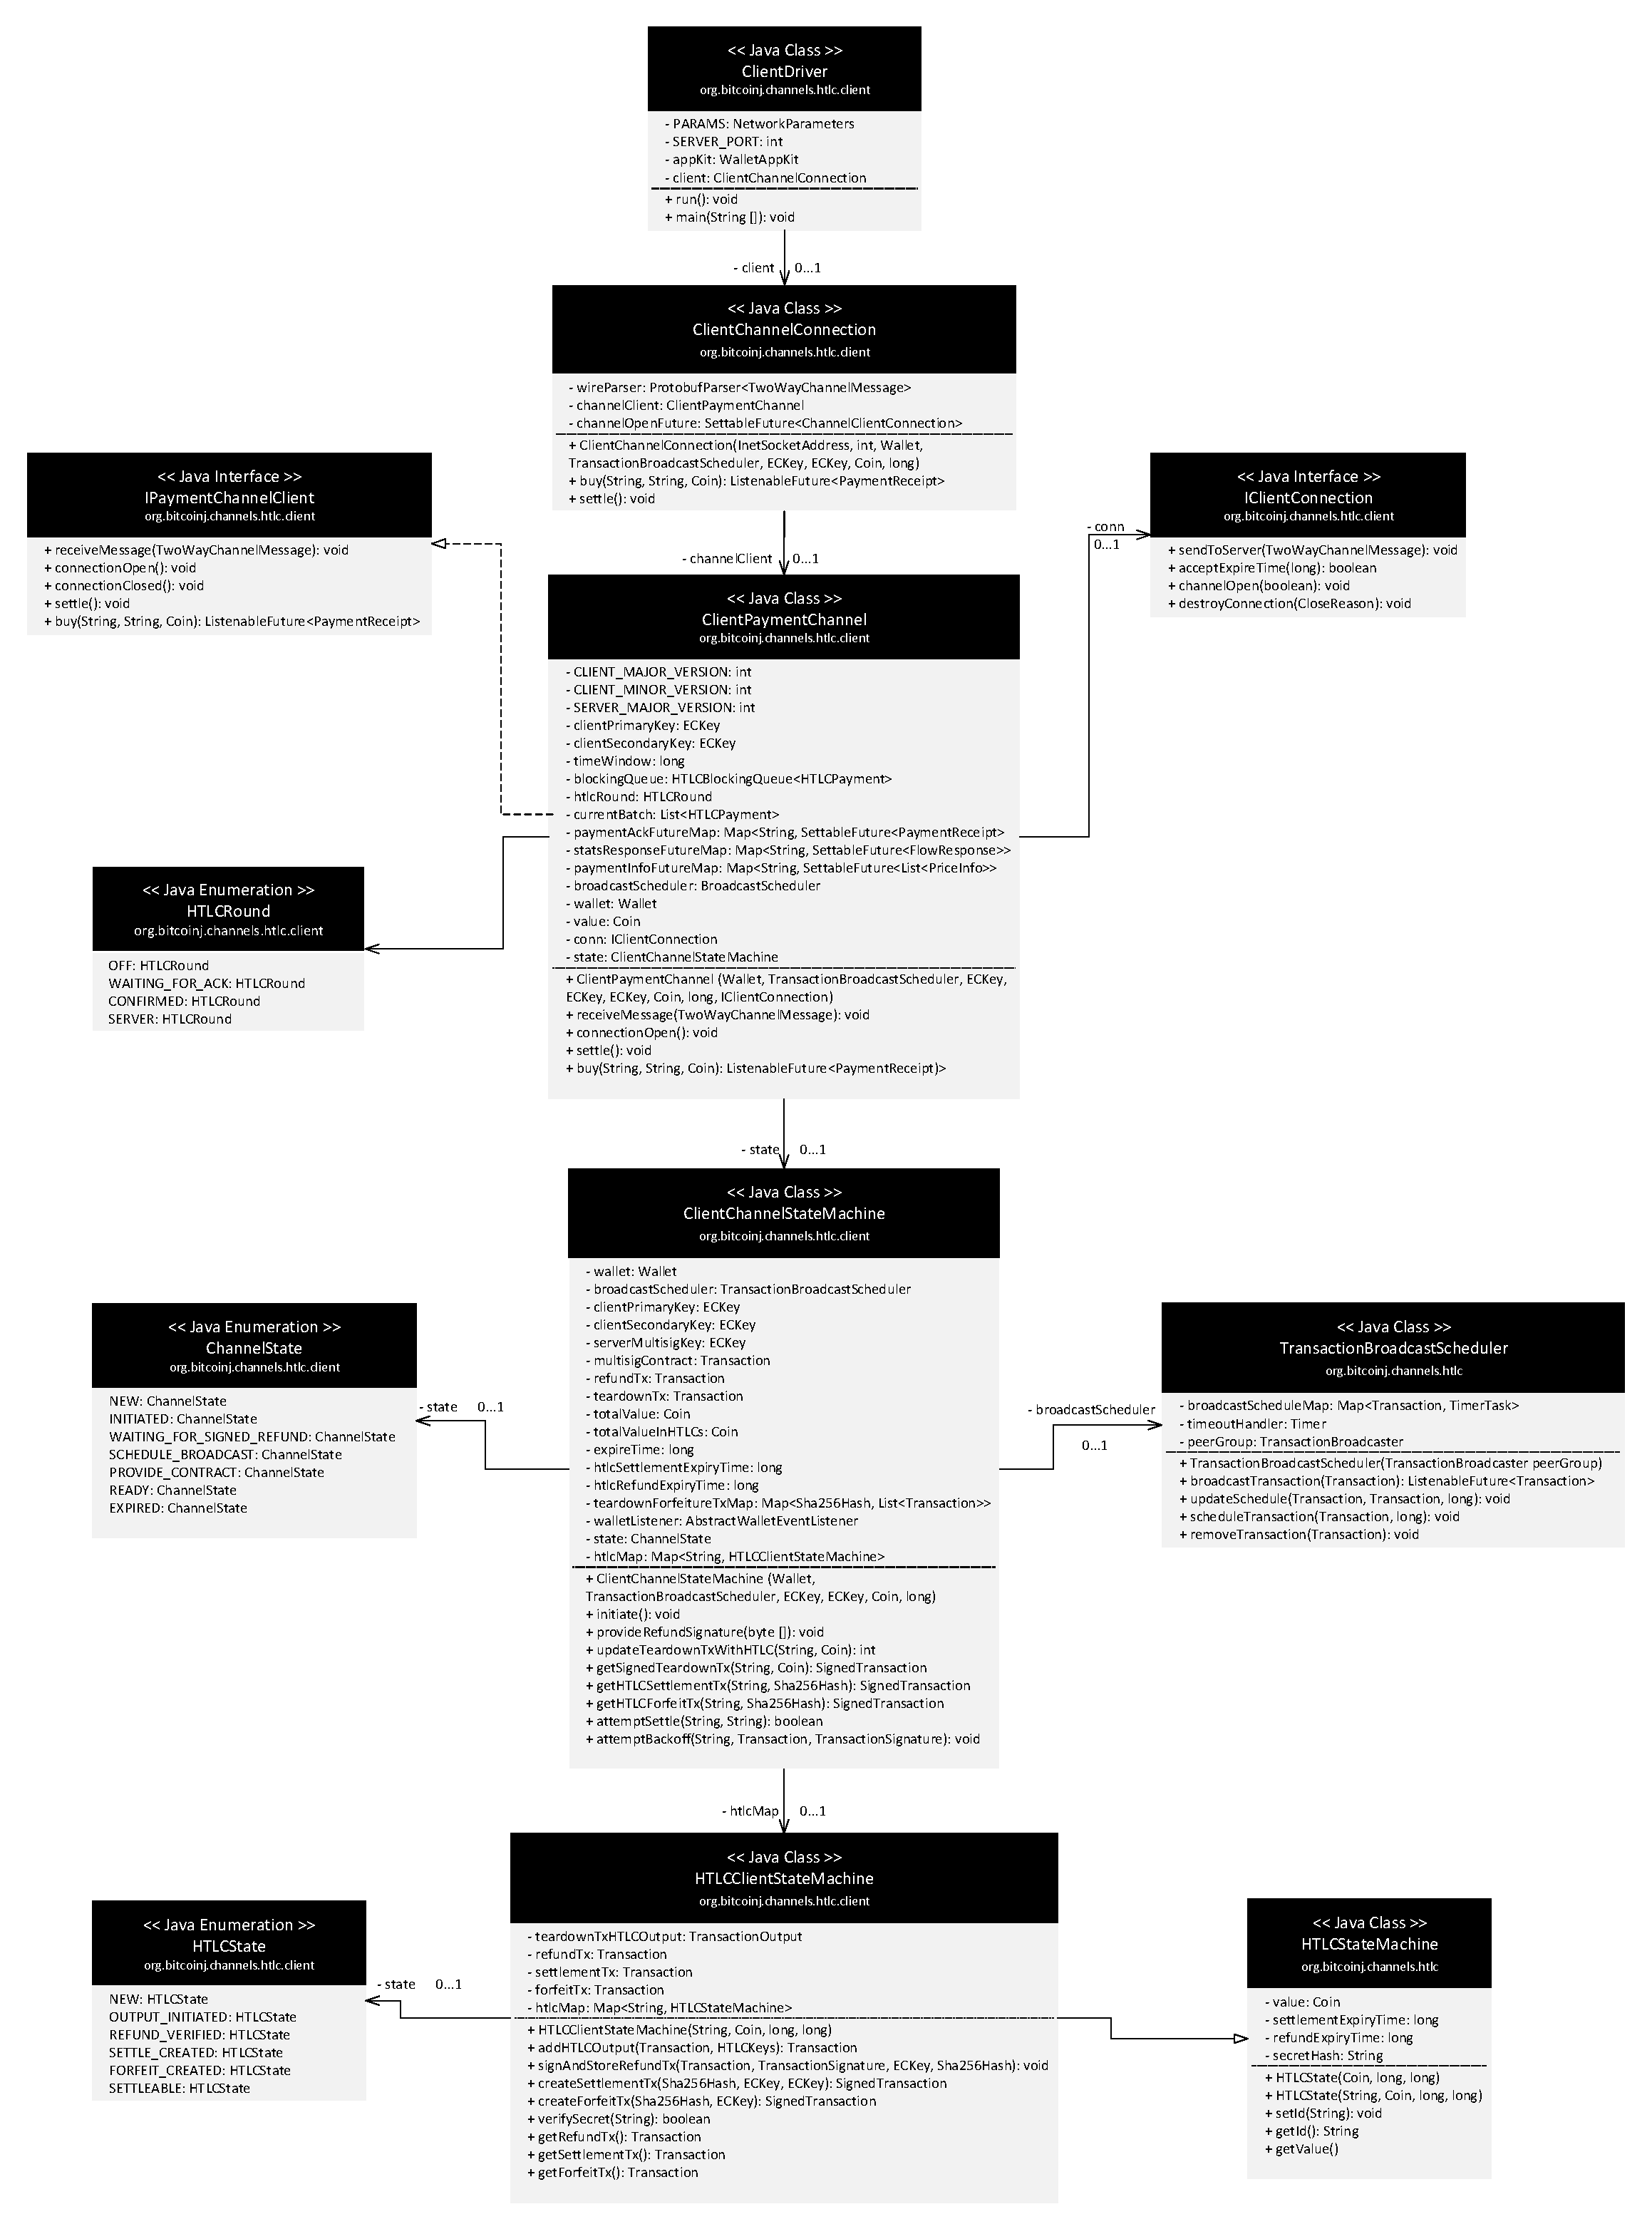
\includegraphics[width=1.2\textwidth]{figures/ClientUML}}
  \caption{UML class diagram of the Client component}
  \label{fig:clientuml}
\end{figure}

The ClientDriver class represents the highest layer in the client application. It instantiates the 
{\it WalletAppKit} object that is part of the {\it bitcoinj} library, which connects to the Bitcoin network and
synchronizes the local blockchain. The driver also loads the wallet of the client, and if the wallet does 
not contain two keys necessary in the protocol participation, it generates them. Once this is completed,
it instantiates the ClientChannelConnection object and calls the method responsible for establishing a micropayment
channel with the server component. As this method triggers a rather long setup process, it is called 
asynchronously, and a callback is registered so the user gets notified once it is completed and payments
can be made through the established channel.

The ClientChannelConnection class is responsible for the communication across the network. Given the address and the port
of the server component, it instantiates the {\it NioClient} object from the {\it bitcoinj} library and connects to it.
The ClientChannelConnection object also creates handlers to events for incoming messages, 
passing them to the lower layer in ClientPaymentChannel for further processing, 
and provides callbacks for events that upper layers can hook up to.

Once messages are passed down to the ClientPaymentChannel class, they are processed by type. When the TCP connection
to the server is established, the micropayment channel setup process is initiated and after an exchange of messages with the
server, payments to it can be made. This class is responsible for analyzing all incoming communication, triggering specific
processes and transitions in lower layers, and ultimately constructing appropriate replies that are sent back to the server.
It implements the IPaymentChannelClient interface that is used by the layer above to pass received messages,
to signal that the connection to the server opened and the micropayment channel setup can be initiated, that a new
payment needs to be made to the server, and that the channel or the connection are closing. Bottom-up communication
between layers is done through the IClientConnection implemented in ClientChannelConnection, 
which enables message sending to the server and callbacks for events such as opening channels and connection abortion.

To provide a safe protocol, it is important to store the progress of establishing a micropayment 
channel so it is always in a secure state. This task is performed by the ClientChannelStateMachine class,
which keeps track of the state the channel is in. It stores the value of the channel, the bond, refund and
HTLC setup transactions, and provides functionality for updating them at appropriate times. 
The TransactionBroadcastScheduler instance field is responsible for scheduling and broadcasting transactions at
the right times, using TimerTasks. Once the channel reaches the {\it ready} state, HTLC payments 
can be made concurrently, which are kept track of using HTLCClientStateMachines. These HTLC state machines provide
methods adding new HTLC outputs to the HTLC setup transaction, attaching refund, settlement, and, if needed,
forfeiture transactions, and lastly, verifying secrets against HTLC hashes. 

\subsection {Server}\label{server}

\hspace*{12pt} Figure \ref{fig:serveruml} shows the structure of the developed server component, 
containing its classes and their relations, attributes, and operations. The classes and their functions 
are described in a top-down manner.

\begin{figure}
  \centerline{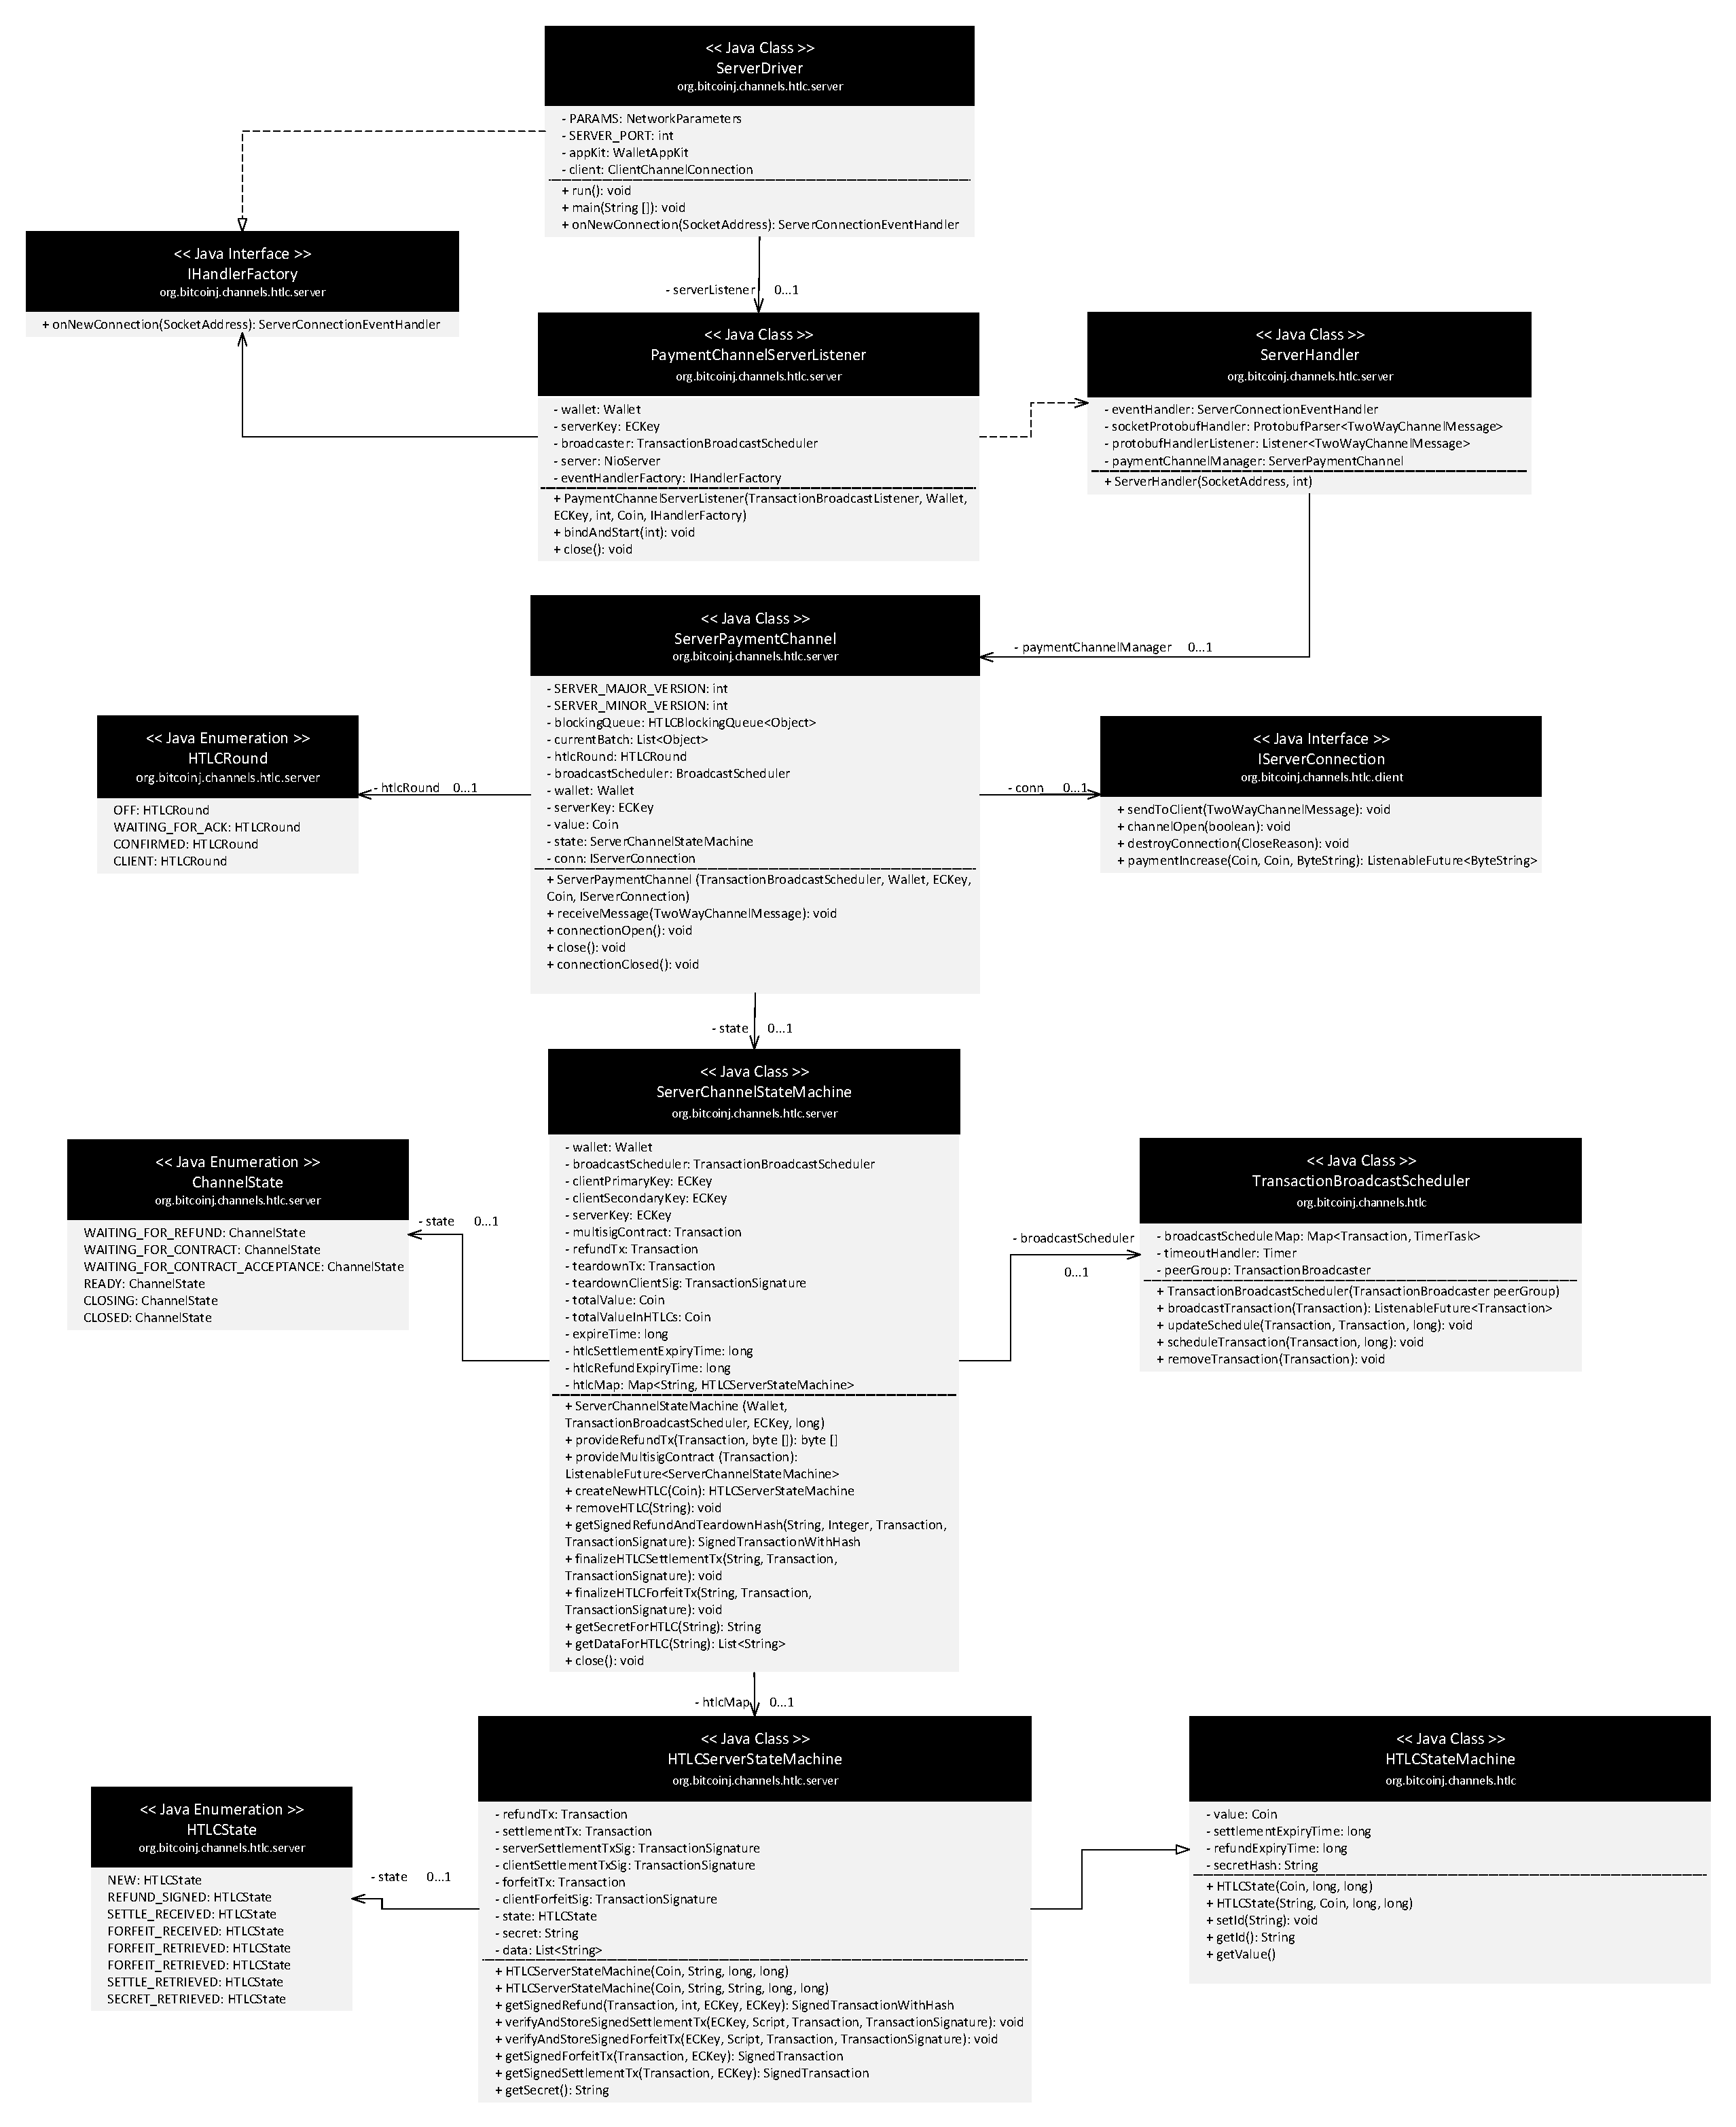
\includegraphics[width=1.2\textwidth]{figures/ServerUML}}
  \caption{UML class diagram of the Server component}
  \label{fig:serveruml}
\end{figure}

Similar to the client side, the ServerDriver class instantiates the {\it WalletAppKit} object that connects to the Bitcoin
network and loads the wallet. After syncing the blockchain, an PaymentChannelServerListener object is created, which 
creates a {\it NioServer} listening on a specified port.

The PaymentChannelServerListener object is responsible for creating ServerHandler instances for each connecting client.
The handler then passes each incoming message to the lower layer for further processing and 
provides callbacks for events such as successfully opening new payment channels or receiving new payments from the client
through the IHandlerFactory interface, implemented in the driver layer. 

Once messages are passed down to the ServerPaymentChannel, they are processed by type, and appropriate actions are taken
in the lower layers. When processing is complete, replies are constructed and sent over to the client side through the 
ServerHandler object, which maintains the TCP connection. Bottom-up calls are done through the IServerConnection 
interface, implemented in the ServerHandler class and passed down to the channel object constructor to be used.

Analogously to the client component, the ServerPaymentChannel stores the state of the channel using a 
ServerChannelStateMachine instance. The state machine keeps track of the value the channel was funded with,
transactions and their time lock expiry and broadcast times. It also provides functions to create, sign, and update
the bond, refund, and HTLC setup transactions. Payment state book-keeping is done using HTLCServerStateMachine objects
stored in a hash map by id. These HTLC state machines provide methods to construct HTLC refund transactions,
verify client signatures on settlement and forfeiture transactions and to sign them with the server key.

\subsection {Cross-component communication}

\hspace*{12pt} System components communicate through TCP connections, transmitting Protocol Buffers (protobuf), 
an extensible, efficient, automated, serialization method introduced by Google in 2008. 
After defining the structure of the data that needs to be serialized through an interface description language, 
a compiler generates source code that allows to write and read the data to in a language independent manner.

To support the proposed payment protocol, the needed data structures were defined using protocol buffer message types
in {\it .proto} files. Each such message contains a series of name-value pairs, associating scalar data types 
with field names. Additionally, each field has an integer field that uniquely identifies it. 
The description language also allows specifying field rules:
\begin{itemize}
 \item {\it optional}: a message containing a field with this rule can contain this field zero zero or one time.
 \item {\it required}: a message containing a field with this rule must contain this field exactly one time.
 \item {\it repeated}: a message containing a field with this rule can contain the field multiple times (including zero).
\end{itemize}

Following the pattern endorsed in the {\it bitcoinj} library, {\it TwoWayChannelMessage}s are extended to support
the communication in the proposed protocol. Below, all used messages are defined using the presented protobuf
description language: all messages prefixed with {\it HTLC*} are introduced for the scope of this work, while the others
already existed in the current version of the library.

\lstinputlisting{protobuf.txt}

The defined messages are received through the {\it receiveMessage()} callback defined in the {\it ProtobufParser} class
in the {\it org.bitcoinj.net} package of {\it bitcoinj}. The ClientConnection object hooks up to this callback
on the client side and ServerHandler on the server side, respectively. 

The next subsections will detail out the use of each message in the micropayment channel setup and HTLC payments.

\subsection {Establishing a micropayment channel} \label{establishmicro}

\hspace*{12pt} Once the TCP connection between the client and the server components is established, 
the client will initiate the process to establish a micropayment channel between the two. 
The exchange of messages in this subprotocol is fully asynchronous to increase throughput and response time.

\begin{figure}[ht!]
  \centerline{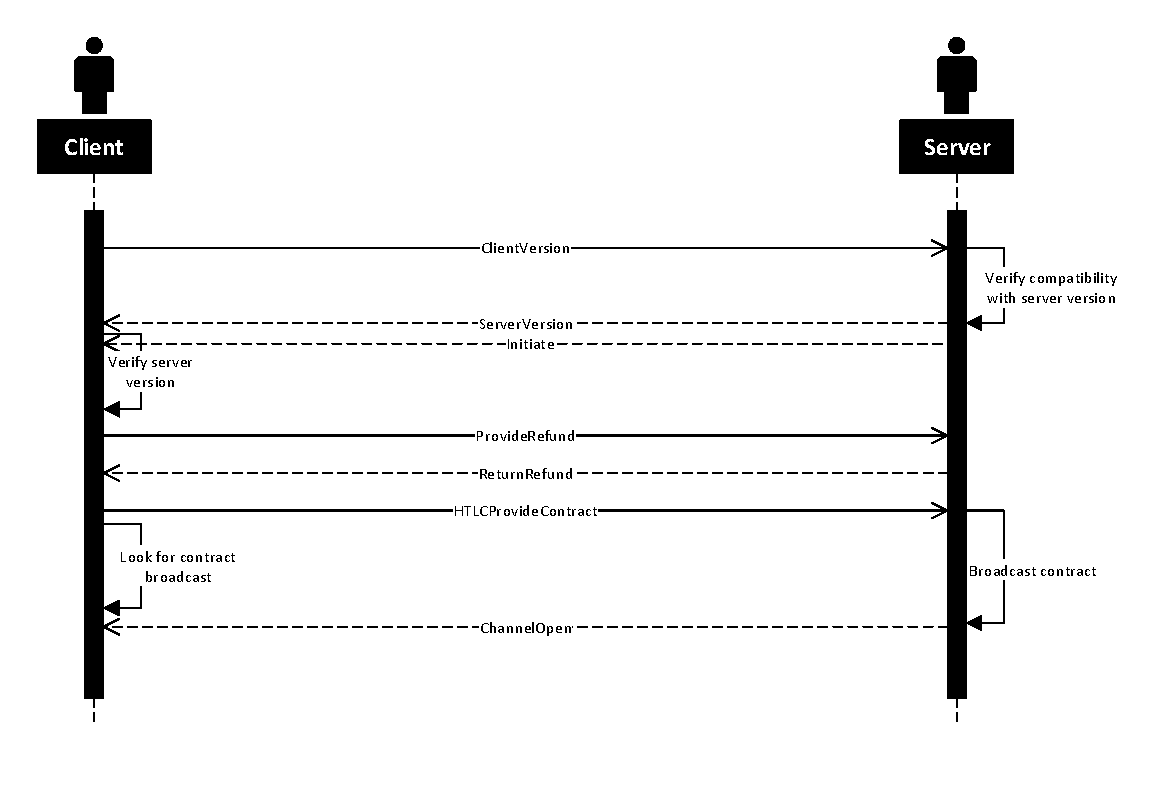
\includegraphics[width=\textwidth]{figures/MicroSeq}}
  \caption{Micropayment channel sequence diagram.}
  \label{fig:microseq}
\end{figure}
\begin{figure}[ht!]
  \centerline{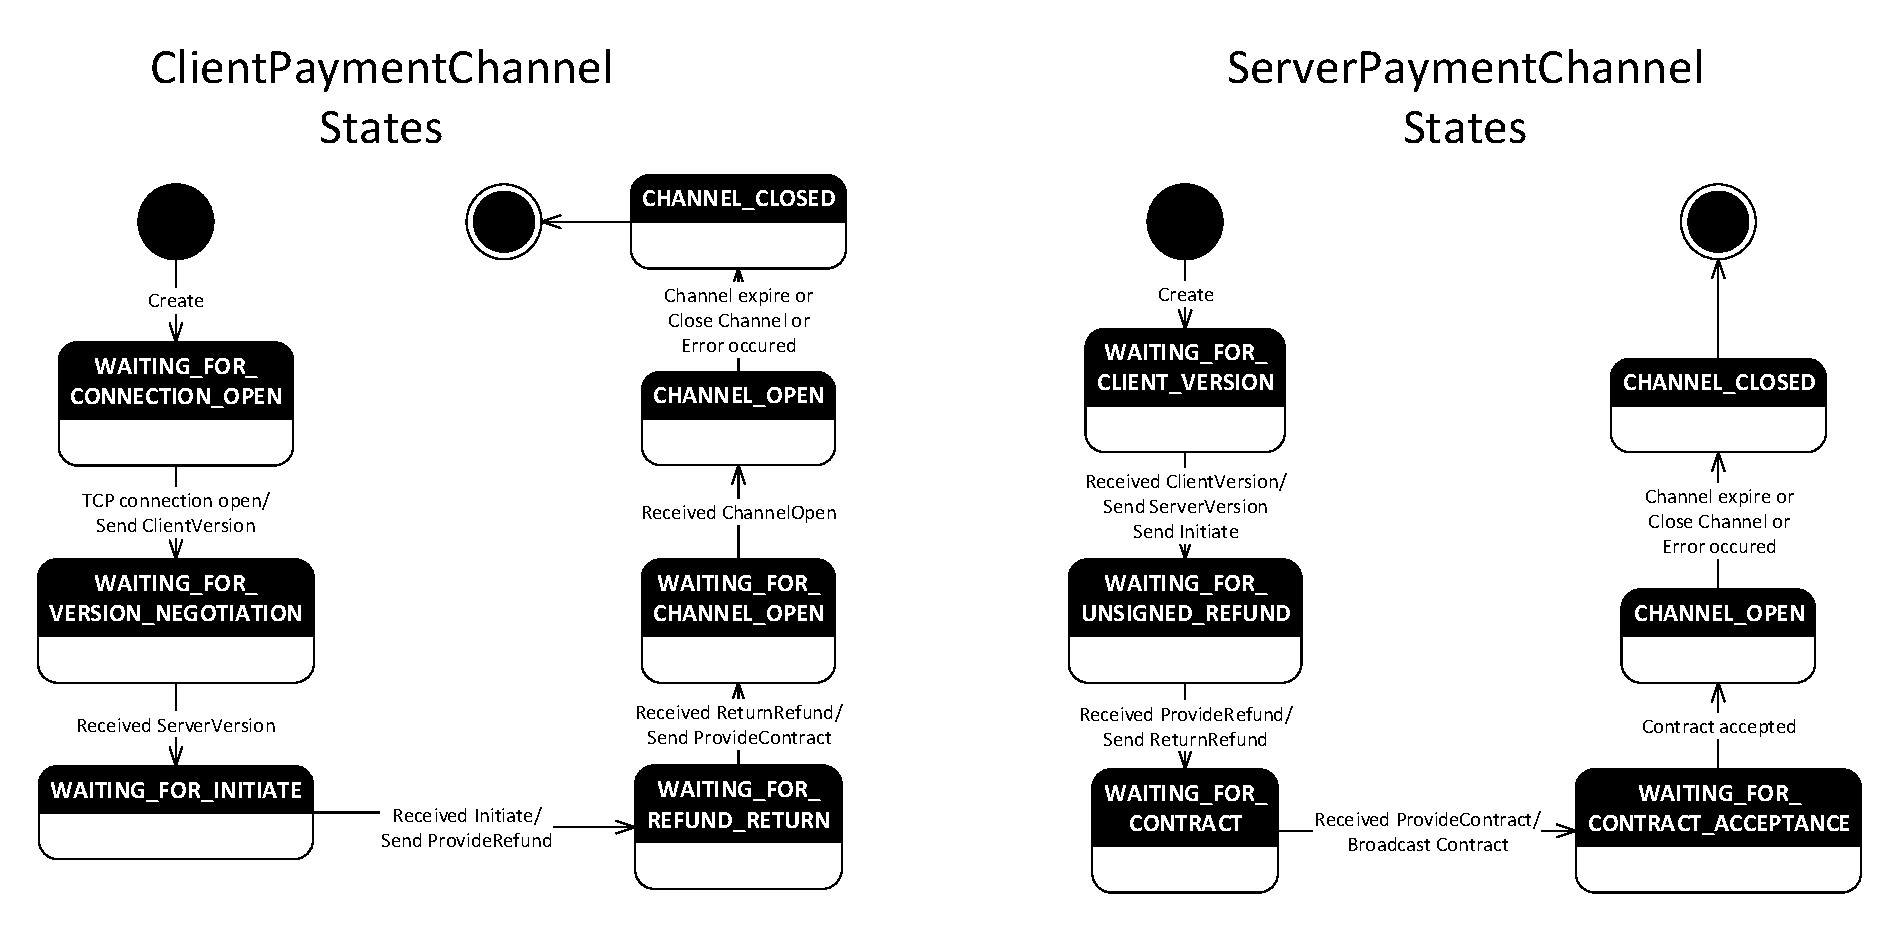
\includegraphics[width=\textwidth]{figures/MicroStates}}
  \caption{Micropayment channel state machine diagram.}
  \label{fig:microstates}
\end{figure}

Figure \ref{fig:microseq} shows the steps and exchange of messages between the client and the server to successfully
set up a payment channel. The logical states of the channel establishment are displayed in 
Figure \ref{fig:microstates}. The transitions correspond to receiving specific messages from the other protocol 
participant. First, the client sends over a ClientVersion message, containing the version of the 
{\it bitcoinj} library it is using, and the time window in seconds the channel should be opened for. The server verifies
if the client version matches its own version, and replies with a ServerVersion message. At this time, the server
also sends the client an Initiate message containing its public key, the expire time of the channel, the minimum
value that needs to be locked into a channel, and the amount of money that the server needs in the initial payment 
for the channel to be opened. The last entry ensures that the client does not open a channel that can not be 
settled because the server received an amount under the dust limit.

When the client receives the Initiate message, it checks that its wallet contains enough funds to open the channel
under the requirements imposed by the server, and instantiates a new ClientChannelStateMachine object, storing
the state of the actual channel. The ClientChannelStateMachine then creates the contract (bond) and the refund
transactions. A ProvideRefund message containing the refund transaction and the public key of the client
is sent to the server. At this point, the server can also create the corresponding ServerChannelStateMachine instance,
it then signs the received refund transaction and returns it to the client in ReturnRefund.

Once it has received the signed refund transaction, the client checks the signature of the server. After
validating it, it creates an initial signed HTLC setup transaction spending from the contract transaction 
a minimum value required by the server, and sends both signed transactions to the server in a HTLCProvideContract
message.

At this point, the server checks the signatures of the client and that the HTLC setup transaction indeed correctly
spends from the contract. After validation, the contract is broadcast to the Bitcoin network.
Once the contract is accepted by the network, the funds of the client are locked in, and the server signals 
the client that the channel is open for payments through a ChannelOpen message.

\subsection {Making an HTLC payment} \label{establishhtlc}

\hspace*{12pt} After a micropayment channel is successfully set up between the client and the server,
the client can begin making small payments in exchange for data. 
When it comes to payments, cross-component communication 
is no longer done asynchronously, but synchronously, using batched update rounds. This solution has been chosen 
to support concurrent payments and is needed so that the HTLC setup transaction is always in a secure and 
consistent state on both the client and server side. Else, updates from both sides could be crossing each other 
and invalidate the signatures of the HTLC refund, settlement, and forfeiture transactions attached to the 
HTLC outputs of the setup transaction.

\subsubsection{Batching and round negotiation}

\hspace*{12pt} Figure \ref{fig:roundneg} shows how update rounds are negotiated between the client and server. 
On the client side, updates are always new payments coming in. On the server side, updates can be of two types:
the server is either claiming an HTLC output by revealing the corresponding secret, or wishes to void an HTLC output.
Both protocol participants buffer update requests in a BlockingQueue while an update round is active.

\begin{figure}[ht!]
  \centerline{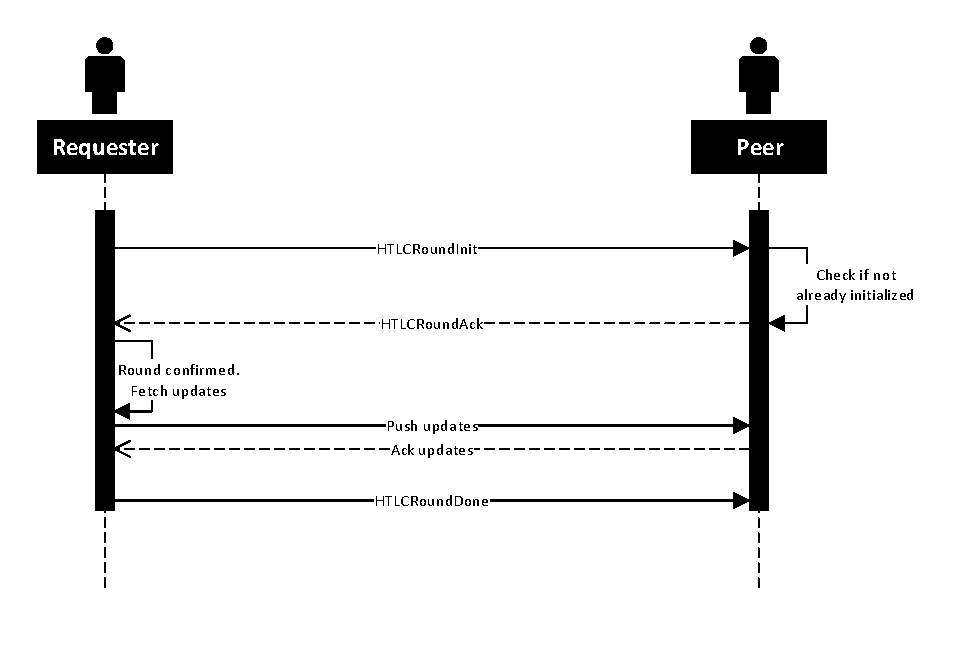
\includegraphics[width=\textwidth]{figures/RoundNegotiation}}
  \caption{HTLC update round negotiation}
  \label{fig:roundneg}
\end{figure}

When one of the components has a new update to push to its peer, it first sends an HTLCRoundInit message to the other
participant. Then, the peer checks if no other update round has been already initialized. If this is the case,
an HTLCRoundAck is sent to the initiator, which confirms the updates can be pushed. In case both participants are
waiting for an HTLCRoundAck message, priority is given to the server. Once the initiator 
finished pushing all updates to the other participant, it marks the end of the round with an HTLCRoundDone message.
If the other participant has buffered updates at this point, it can now safely initiate its own update round.

\subsubsection{Initiating a payment} \label{initpay}

\hspace*{12pt} After the client has secured an update round through the negotiation mechanism presented above, 
it can send new payments to the server. The full process is shown in Figure \ref{fig:htlcsetupseq}.

\begin{figure}[ht!]
  \centerline{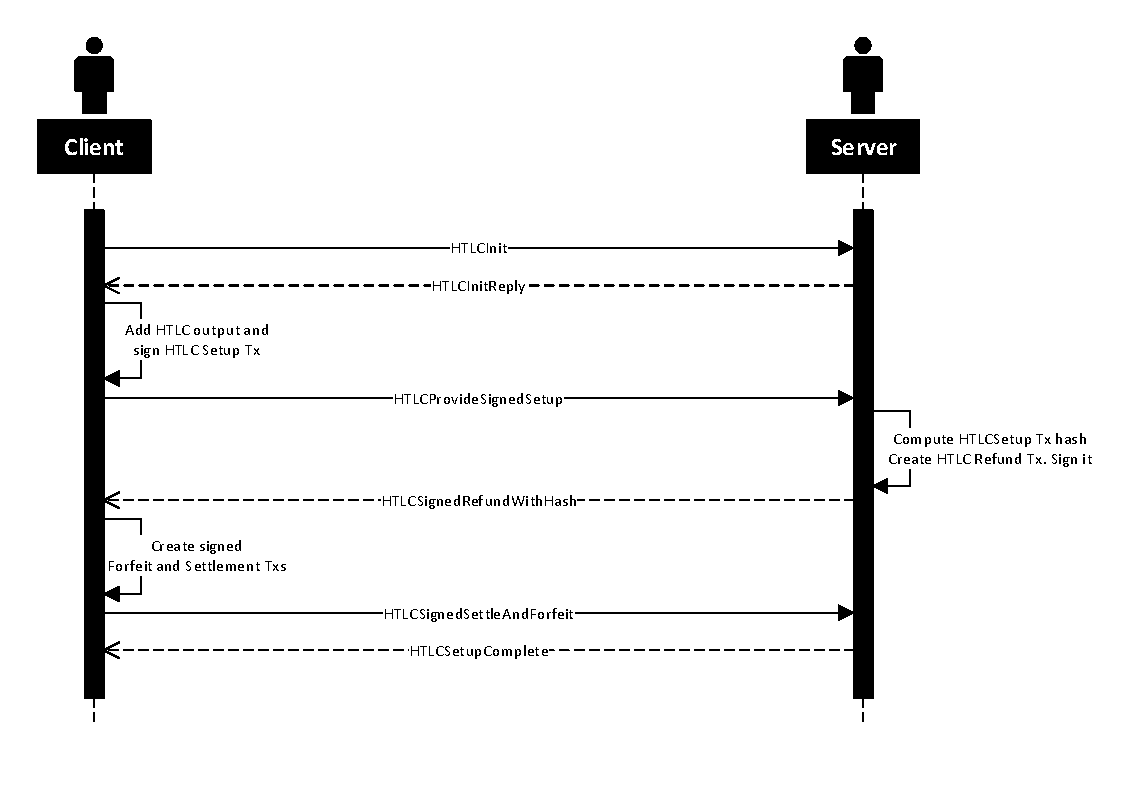
\includegraphics[width=\textwidth]{figures/HTLCSetupSeq}}
  \caption{HTLC Setup sequence diagram}
  \label{fig:htlcsetupseq}
\end{figure}

\begin{figure}[ht!]
  \centerline{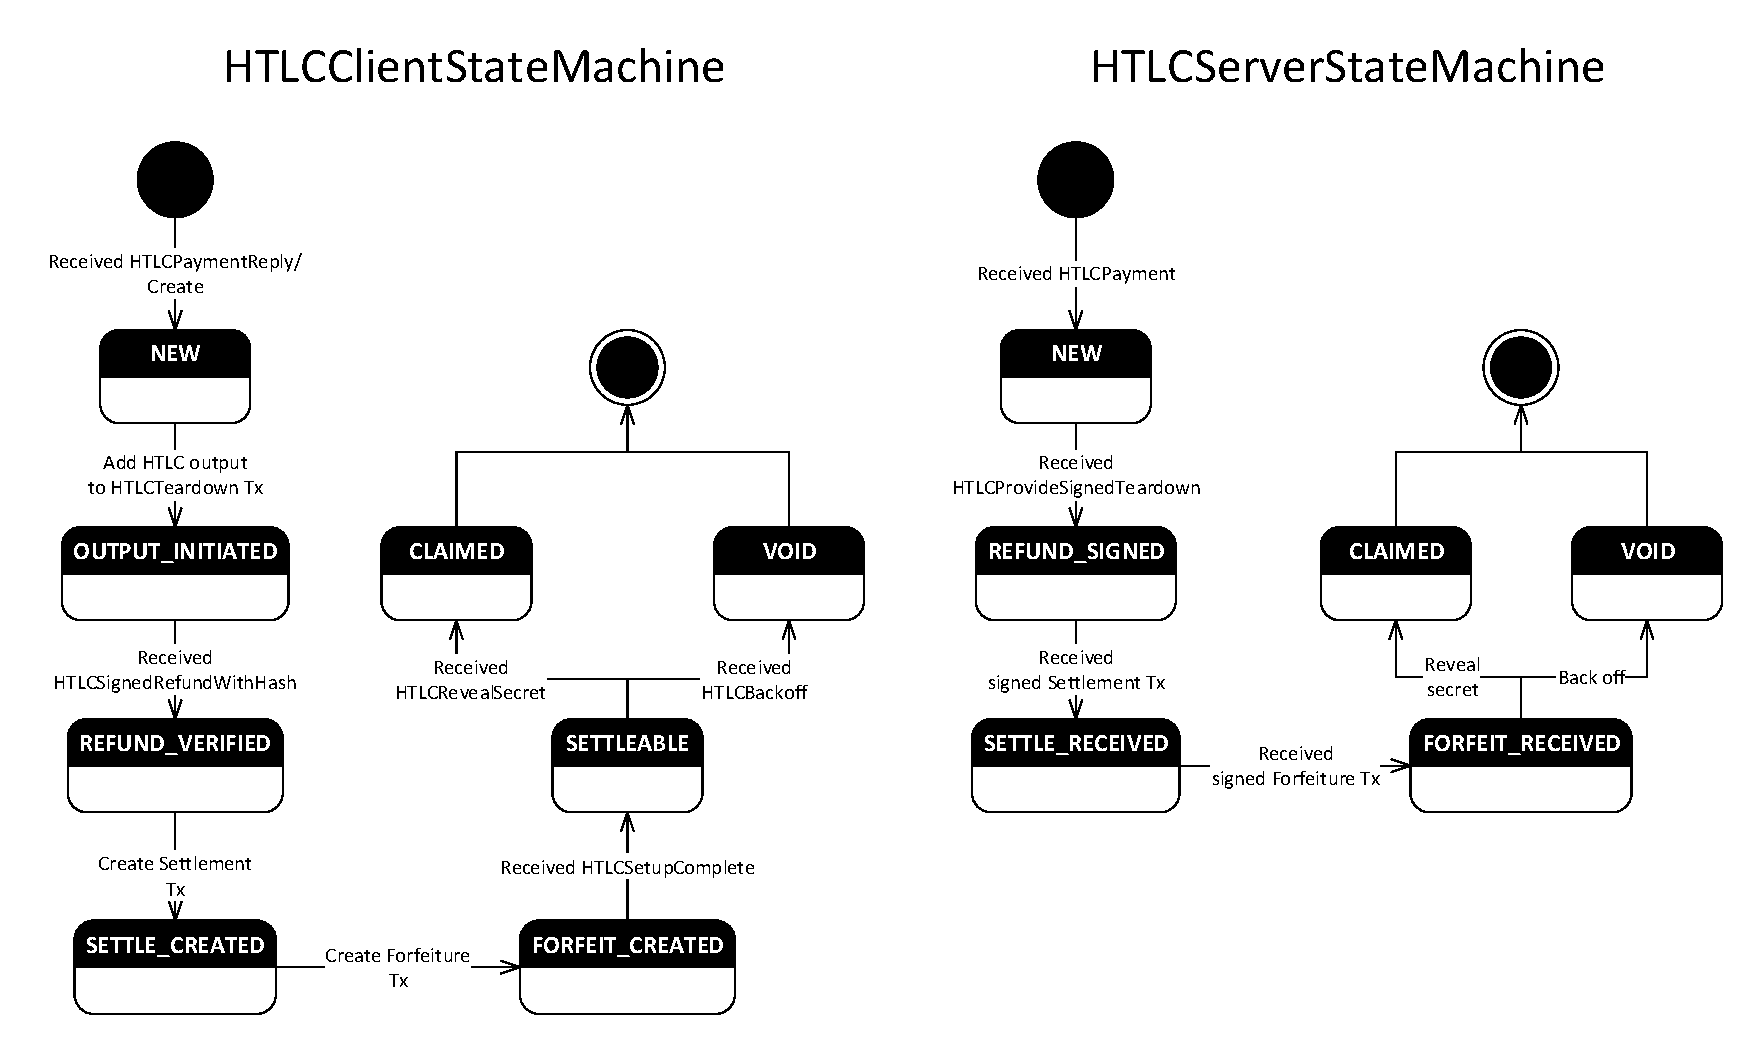
\includegraphics[width=\textwidth]{figures/HTLCStates}}
  \caption{HTLC State Machines for both client and server side}
  \label{fig:htlcstates}
\end{figure}

The client first sends an HTLCInit message containing a list of payments that were buffered during a previous active round.
Each payment message contains a client request id, the value of the payment and information about the type of data that
is requested in exchange. The server creates new HTLCServerStateMachine instances for each payment. Each HTLC is given an id,
which is basically the hash of the secret. An HTLCInitReply message is then replied, mirroring back the client request id,
and sending the fresh HTLC id. From this stage on, each HTLC payment will be referenced by the server-generated id.

At this stage, the client can also create HTLCClientStateMachine instances and update the HTLC setup transaction, adding
it outputs for each initiated payment. The transaction is then signed and sent over to the server, together with the 
payment ids and indexes of each payment output.

Because of the Bitcoin malleability issue, this step in the protocol has a major caveat: it sends over the signed 
HTLC setup transaction before having any signed HTLC refund transaction that protects the client in case the server
decides to lock away the funds in the HTLC outputs indefinitely. It can not be avoided without the malleability fix,
because the client can not create by itself an HTLC refund transaction that spends from the HTLC output:
the HTLC setup transaction spends from the multisig output between the two parties, and it needs to be fully signed
for the refund transaction to correctly reference it by its hash. Thus, in the current implementation, a minimal amount
of trust is needed in the server component, that it will indeed sign, compute the hash of the HTLC setup transaction,
and return signed HTLC refund transactions for all active HTLC payments (HTLCSignedRefundWithHash). 
This step is necessary because removing outputs from the HTLC setup transaction invalidates the signatures 
of previously created HTLC refund, settlement and forfeiture transactions.The amount of trust
can be adjusted by limiting the number of active HTLC payments at a time.

Once the client received the HTLC setup transaction hash and HTLC refund transactions for each payment, 
the protocol is back to a secure state. The client can now recreate the HTLC forfeiture and settlement transactions
for all active HTLC payments, sign and hand them over to the server.After the server checks the signatures and stores the 
received transactions, it will signal the client that the HTLC setup is complete.

\subsubsection{Claiming a payment}\label{claim}

\hspace*{12pt} After a successful setup, the server can initiate an update round to claim the payments from the HTLC outputs.
To do so, it first sends an HTLCServerUpdate message to the client. It contains a list of HTLCRevealSecret 
and a list of HTLCBackoff messages. Each reveal message indicates the id of the HTLC payment the server is claiming,
together with the secret that hashes to its id. Back-off messages are sent by the server a fixed time before the 
channel expiration time and before the HTLC setup transaction is broadcast, such that the number of HTLC refund transactions
that are later broadcast by the client is minimized. Thus, the refund transactions are kept off the blockchain, and
the server voluntarily opts to void the HTLC payments because it has not received the secret in time. 
Together with the ids of the HTLC payments that are voided, the server sends over the fully signed HTLC 
forfeiture transaction, which guarantees the client that an older HTLC setup transaction will not be broadcast, 
should the secret be received at a later time. 

\begin{figure}[ht!]
  \centerline{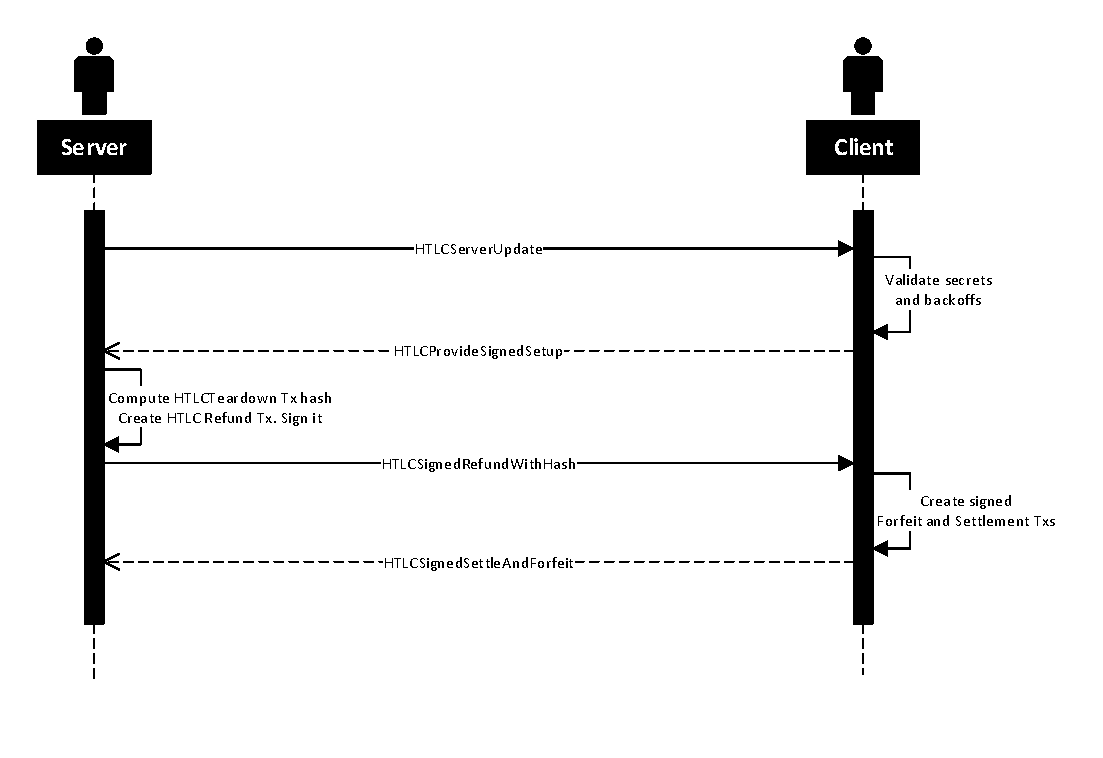
\includegraphics[width=\textwidth]{figures/HTLCClaimSeq}}
  \caption{HTLC Claim and Backoff sequence diagram}
  \label{fig:htlcclaimseq}
\end{figure}

The client validates the reveal secrets and forfeiture transactions, and removes the HTLC outputs from the HTLC 
setup transaction accordingly. Forfeiture transactions are stored and hashes of older
HTLC setup transactions are followed on the blockchain. Should any of them make it to the blockchain,
the client will automatically broadcast the corresponding forfeiture transactions to get the funds back.
The updated HTLC setup transaction is then signed sent to the server using the HTLCProvideSignedTeardown message. 
From here on, the process follows the same steps as in \ref{initpay}. 
The message succession is shown in Figure \ref{fig:htlcclaimseq}. 

\subsubsection{Data transmission}

\hspace*{12pt} In order to securely transmit the data that the client is issuing payments for, the client and the server needs
a private, authentic out-of-band channel. In the HTLC payment setup phase, the data, encrypted with the HTLC secret,
would be transmitted to the client using this channel. Then, once the server has cleared the payment by revealing the secret,
the client can decrypt the previously received data. This ensures an atomic exchange of data for bitcoins.

\section {Application implementation}

\hspace*{12pt} Following the design introduced in the previous chapter and the client-server architecture described in the 
previous section, three different applications were developed, corresponding to each of the three components: 
buyer, central hub, and sensor node represented by an Android application on a device with a wide range 
of built-in sensors. In the next subsections, each application is presented in detail.

\subsection{Buyer application}

\hspace*{12pt} The buyer component was developed as a Java console application. From an architectural point of view,
it plays the role of a client in the payment protocol by connecting, initiating a micropayment channel with the hub and 
making payments to the hub in exchange for data.

\subsubsection{Running queries}
\hspace*{12pt} From the buyer driver console application, the following queries are available:
\begin{itemize}
 \item Node statistics. {\it STATS NODES} will display the number of connected sensor nodes with 
 list of sensor node ids. 
 \item Sensor statistics. {\it STATS SENSORS} will display the types of sensors that are available for purchasing.
 \item Select queries. {\it SELECT SENSOR=\textless sensor\_type\textgreater } will display 
 all available nodes with the selected sensor type, together with id of the node it is available on, 
 and pricing information,
 \item Buy queries: {\it BUY \textless sensor\_type\textgreater FROM node\_id price} will 
 purchase the set of sensor data of the specified type from the node selected by id. 
 This query will return the asked data set.
\end{itemize}

\subsection{Hub application}

\hspace*{12pt} The hub application was developed as a Java application. It represents the discovery, coordination and payment
forwarding point of the developed system, with both a receiving (server) component from the perspective of the 
buyers, and a sending (client) component from the perspective of the sensor nodes.

\begin{figure}[ht!]
  \centerline{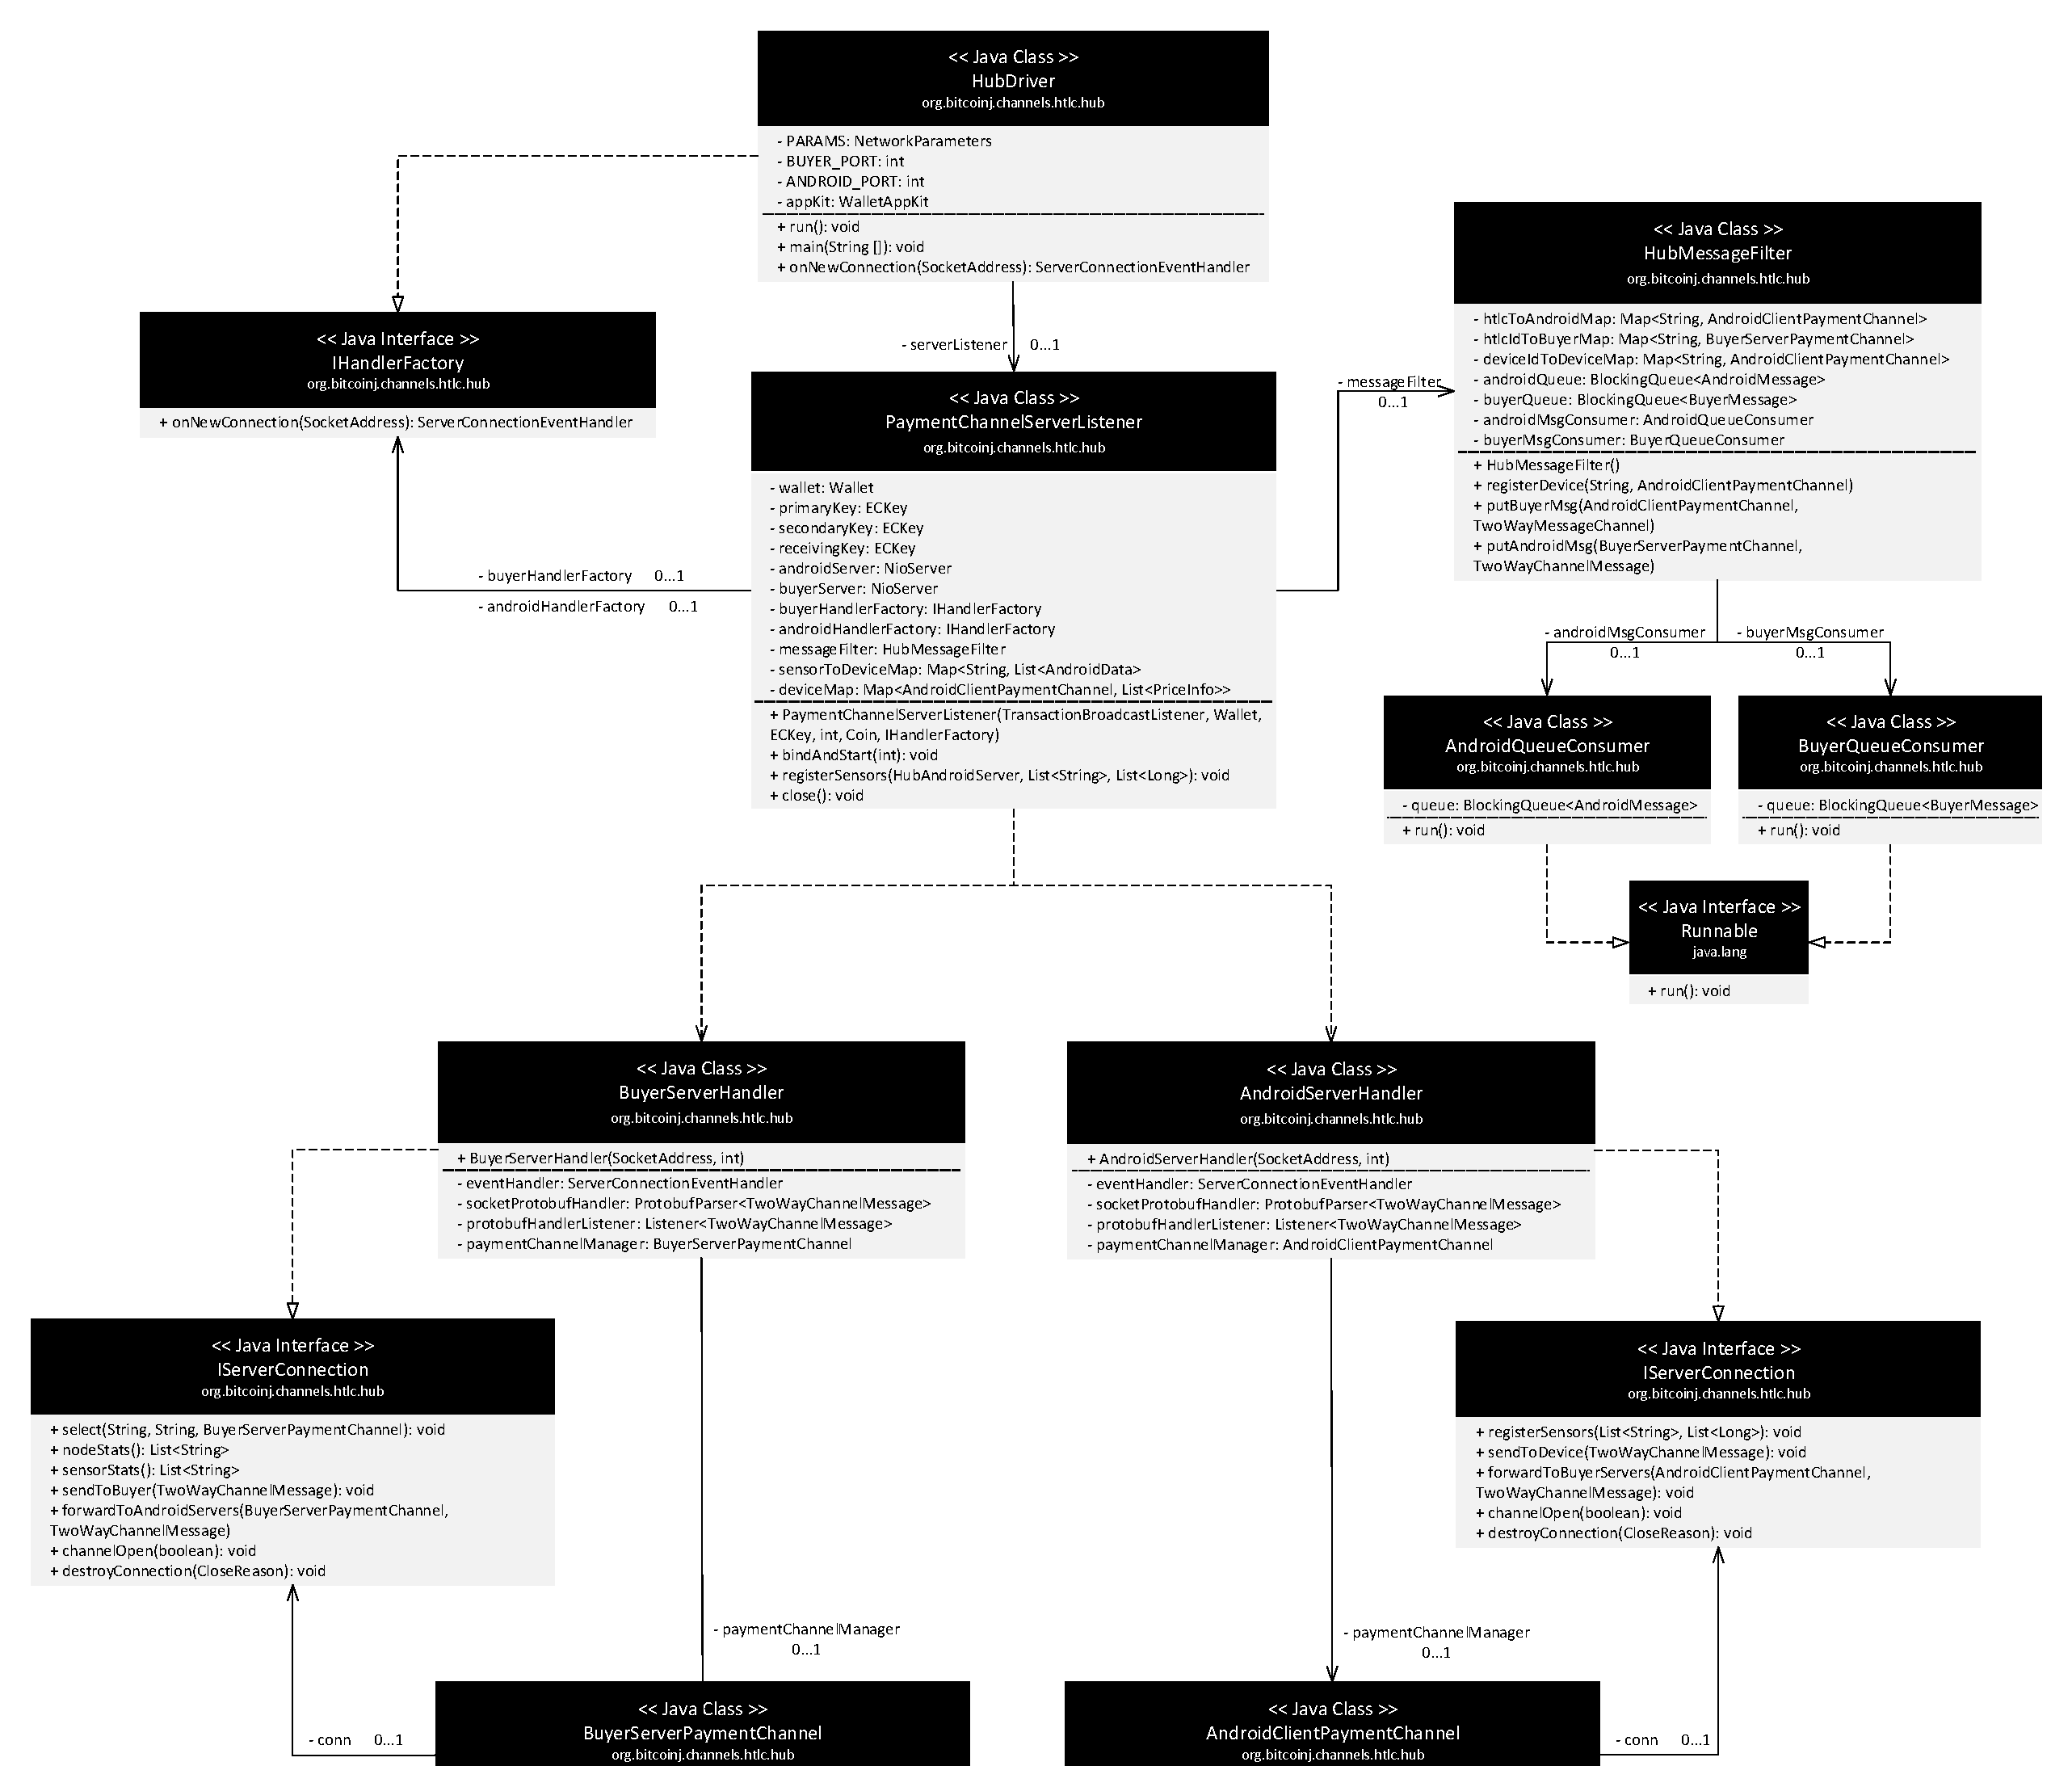
\includegraphics[width=1.25\textwidth]{figures/HubUML}}
  \caption{Hub class diagram of the first three layers.}
  \label{fig:hubuml}
\end{figure}

Figure \ref{fig:hubuml} shows the structure of the developed hub component, containing the classes and their
relations, attributes, and functions from the DriverApplication, ChannelConnection, and PaymentChannel layers. 
The ChannelStateMachine and HTLCStateMachines layers were integrated as originally designed.

The HubDriver class instantiates the Bitcoin related objects, and launches the PaymentChannelHubListener, the class
responsible for running two NioServers on two different ports: one for connecting buyers, and another one for sensor nodes.
It also stores data such as mappings of sensor types to the devices that they are installed on, and pricing information,
such that it can support node, sensor, and select queries. 

The HubMessageFilter object associated to the listener class keeps track of all payment ids and of the buyers
and sensor nodes these payments are initiated between. This way, the destination of messages that need to be 
forwarded between the buyer and the Android components can be easily identified. If a message contains sub-messages
for multiple destinations, the filter does deep-packet inspection, aggregates the sub-messages by destination, and finally
forwards them.

When a buyer connects to the hub, the buyer NioServer object instantiates a new BuyerServerHandler. This creates 
a new BuyerServerPaymentChannel, which is basically a ServerPaymentChannel object as introduced in \ref{server}
supporting statistical node and sensor queries, and forwarding to the Android payment channels through the 
nested IServerConnection interface.

When a new device connects to the hub, the Android NioServer instance creates an AndroidServerHandler. This component
instantiates a new AndroidClientPaymentChannel, which is simply a ClientPaymentChannel object previously 
introduced in \ref{client}, with additional support for forwarding messages to the Buyer payment channels. 
To forward messages to buyers, the {\it forwardToBuyerServers()} method from
the nested IServerConnection interface can be used, which calls all the way up to the listener class and dispatches
the job to the HubMessageFilter.

The functionality of the lower layers introduced in the client-server protocol design is fully preserved.

\subsection{Android application}

\hspace*{12pt} The sensor node component was developed as an Android application, allowing the user of the app
to share sensor data in exchange for bitcoins. Since it represents the receiving party in the protocol,
it follows the server component design.

\begin{figure}[ht!]
  \centerline{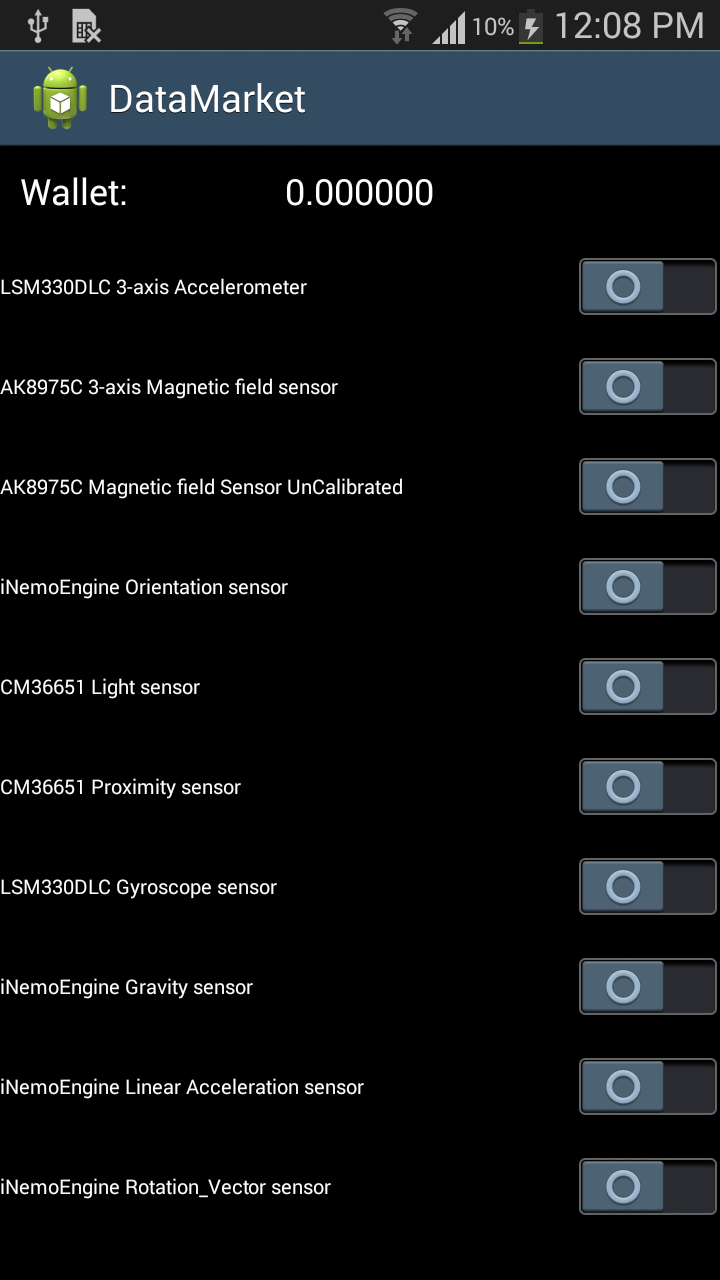
\includegraphics[width=.5\textwidth]{figures/app}}
  \caption{Android application user interface.}
  \label{fig:app}
\end{figure}

The user is given full choice regarding which data is shared to the interested buyers. The available device sensors
are detected at application start-up. The interface (Figure \ref{fig:app})
consists of a main view that allows the user to toggle between sharing or not sharing the data of each sensor.

The Bitcoin wallet is created on the first start and locally stored on the device. At this time, the user
can also set up prices for sensor sharing. At the top of the interface, the application displays 
the amount of bitcoins earned so far.

\subsubsection{ChannelConnection layer adaptation}

\hspace*{12pt} In the original design, the ChannelConnection layer of the server is the one listening for new connections
from connecting clients. However, in this case, the Android application should be the one initiating the connection 
and registering to the central hub. In this regard, the ChannelConnection layer was adapted such that app is the one 
initializing the connection (connection client), but the payment protocol message exchange stays the same: 
the Android component is the receiving party, thus a payment server component.

\subsubsection{Connectivity}

\hspace*{12pt} To establish and maintain the TCP connection to the Hub, the code responsible for the Bitcoin operations was integrated
into an Android remote service that starts at device boot-up. This ensures that the long-running operations do not block
the application user interface and that the micropayment channel is kept alive even if the user closes the application.

To ensure the communication between the Android activity classes and the remote service, AIDL (Android Interface Definition
Language) was used. Using AIDL, two interfaces have been defined:

\hspace*{1pt}
\lstinputlisting{aidl.txt}

Once the remote service is created, the main application can bind to it, which returns an object 
implementing the HTLCServiceApi interface. Using it, the activity class can register an object implementing
the HTLCServiceListener interface to the service through the {\it addListener()} method. Thus, the two-way binding
is complete.

When the service successfully establishes the TCP connection and sets up a micropayment channel with the hub,
the application is signaled through the {\it channelEstablished()} method. Then, the application registers the shared
sensors to the hub using {\it updateSensors()}. This is repeated every time the user changes its preferences 
in terms of the sensors data that is shared.

When the buyer requests some data from a specific sensor through the hub, the remote service can use
{\it getDataFromSensor()} to retrieve the data from the sensor listeners running in the application. 
Sensor listeners cache the data to allow instant data retrieval. A {\it DataContainer} class customizes the
number of data entries that are cached. The current implementation uses a EvictingQueue of a fixed size {\it K},
automatically maintaining the {\it K} most recent entries.

\subsubsection{Permission requirements}

\hspace*{12pt} The following Android permissions need to be granted in order for the device to successfully participate
in the built system:
\begin{itemize}
 \item {\bf android.permission.INTERNET}. The application needs Internet connectivity at all times.
 \item {\bf android.permission.WRITE\_EXTERNAL\_STORAGE}. The application needs permission to store and update the wallet
 and blockchain files.
 \item {\bf android.permission.RECEIVE\_BOOT\_COMPLETED}. The application needs to receive the BOOT\_COMPLETED signal
 to initialize the micropayment channel to the hub.
\end{itemize}

\subsection{Running the full-system protocol}

\begin{figure}[ht!]
  \centerline{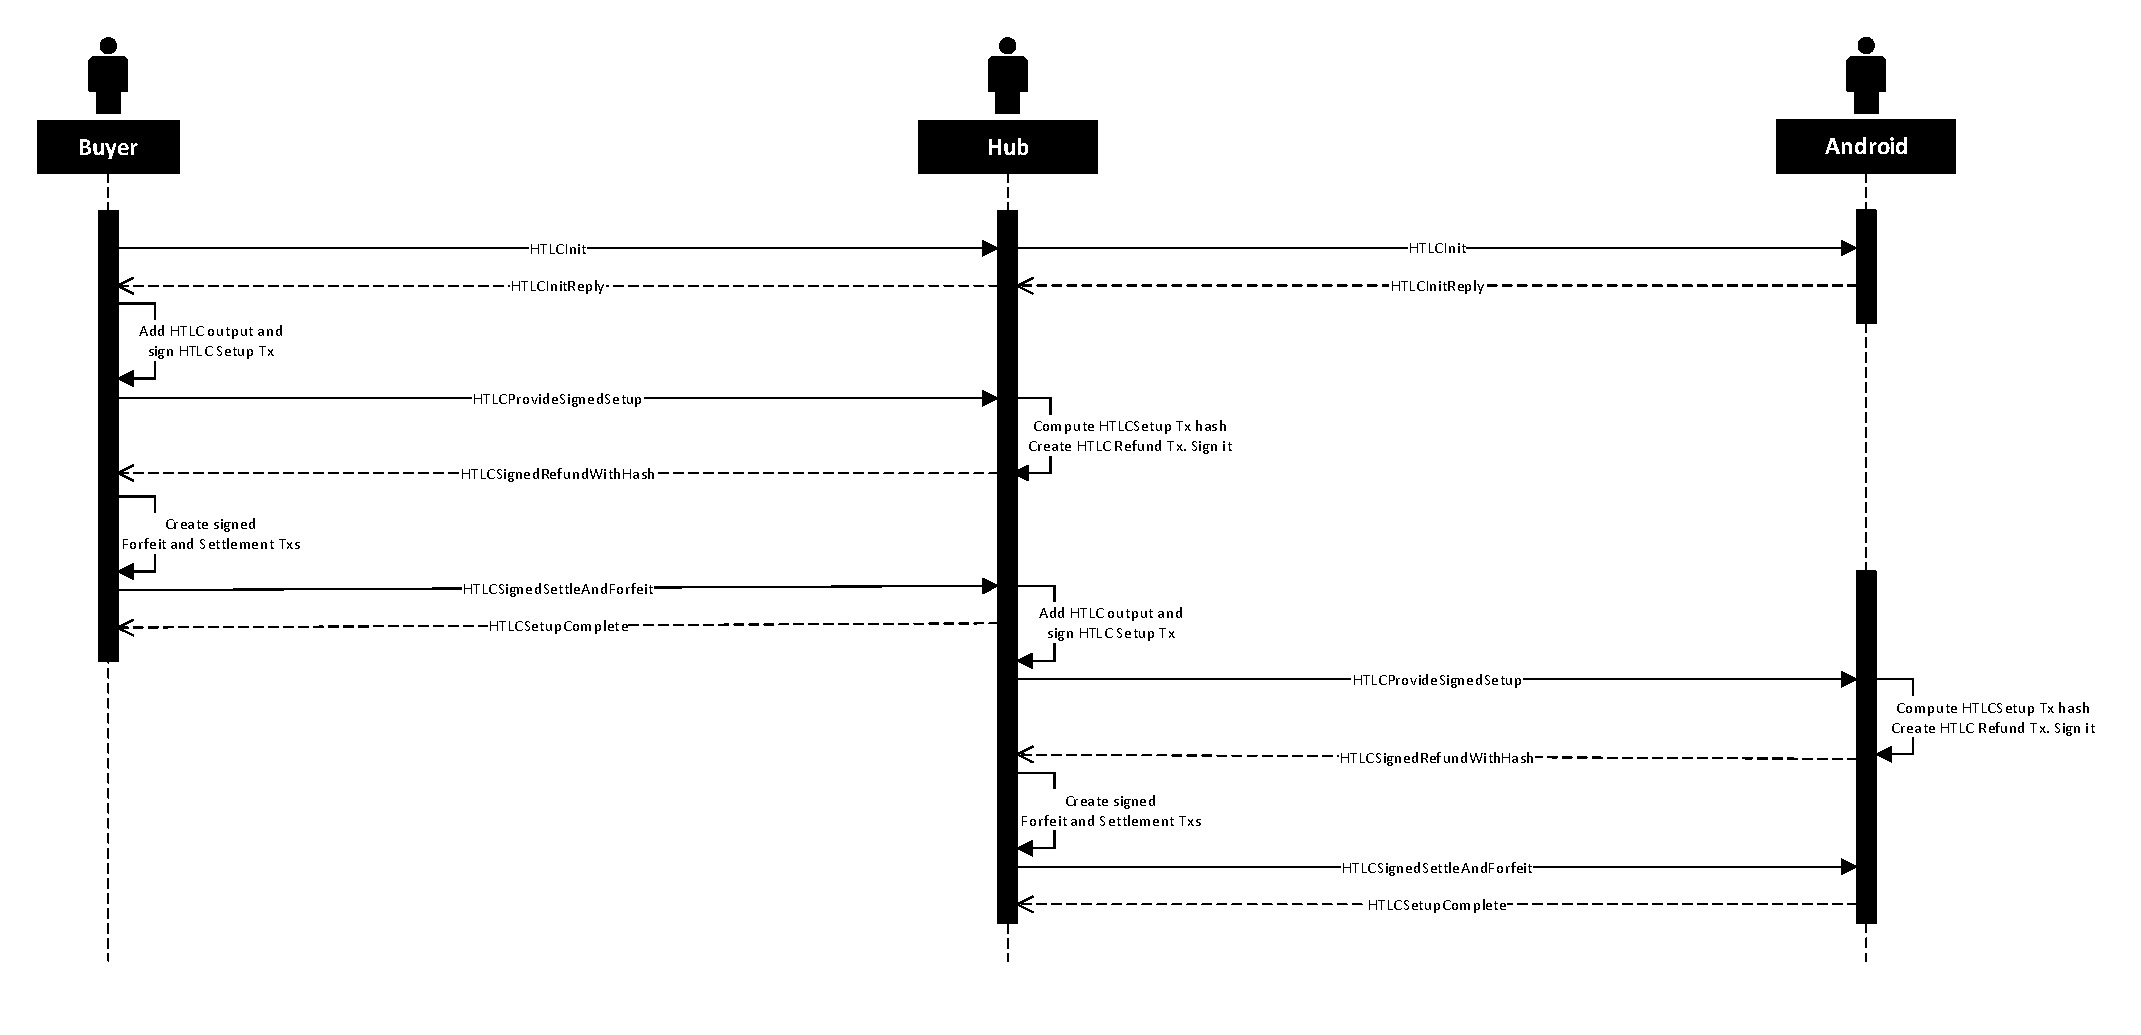
\includegraphics[width=1.5\textwidth]{figures/FullHTLCSetup}}
  \caption{HTLC Full Setup sequence diagram}
  \label{fig:htlcfullsetup}
\end{figure}

\hspace*{12pt} In the full, three-component system, micropayment channels between the participants are 
established independently. Once at least one buyer and one Android device are connected and channels are in place, 
the buyer can initiate payments and receive the requested data in return. All requests are made during batched
update rounds.

Figure \ref{fig:htlcfullsetup} shows the message succession needed for the HTLC payment setup. First, the buyer sends an HTLCInit
message. Upon receiving it, the BuyerServer forwards the message to the AndroidServer through the HubServerListener object.
The AndroidServer then sends the HTLCInit to the AndroidClient, which replies with an HTLCInitReply message. At this stage,
the AndroidServer does not continue running the setup protocol, but forwards back the reply, finally making it to the 
payment initiator. Now the buyer and the BuyerServer subcomponent of the hub can run the HTLC payment setup protocol
presented in detail in \ref{initpay}. 

After a successful setup, the BuyerServer signals the AndroidServer
that it can resume the paused setup protocol with the AndroidClient through the HTLCResumeSetup message. It is important
that the HTLC payment is first set up between the buyer and the BuyerServer to ensure the security of the protocol:
should the AndroidServer and the AndroidClient first set up such a payment, nothing guarantees the AndroidServer
that it can claim the money from the buyer after it has paid the AndroidClient.

When the AndroidClient claims or voids some HTLC payments, it follows the exact pattern introduced in \ref{claim}.
Only this time, after the AndroidServer receives and validates the HTLCServerUpdate message, it forwards it immediately
to the BuyerServer, and then continues with its update round. This way, the BuyerServer can also run the update protocol
simultaneously and the BuyerClient can use the secret to decrypt the received data that was included in the HTLCInitReply
message.

\chapter{Evaluation}

Notes: - talk about data = rubbish - reputation system needed as in ebay, amazon, etc.
- add bitcoin malleability issue
- data encryption options and integrity with hmac (requires shared secret)

\chapter{Conclusion}

\chapter{References}

% This displays the bibliography for all cited external documents. All references have to be defined in the file references.bib and can then be cited from within this document.
\bibliographystyle{splncs}
\bibliography{references}

% This creates an appendix chapter, comment if not needed.
\appendix
\chapter{Appendix Chapter}

\end{document}